% Created 2016-02-02 Tue 19:22
\documentclass[journal=jpccck,manuscript=suppinfo,email=true]{achemso}
  \setkeys{acs}{biblabel=brackets,super=true,articletitle=false}
\SectionNumbersOn
\usepackage[utf8]{inputenc}
\usepackage{fixltx2e}
\usepackage{url}
\usepackage[version=3]{mhchem}
\usepackage{graphicx}
\usepackage{float}
\usepackage{color}
\usepackage{amsmath}
\usepackage{textcomp}
\usepackage{wasysym}
\usepackage{latexsym}
\usepackage{amssymb}
\usepackage[linktocpage, pdfstartview=FitH, colorlinks, linkcolor=black, anchorcolor=black, citecolor=black, filecolor=black, menucolor=black, urlcolor=black]{hyperref}
\usepackage{attachfile}
\usepackage{longtable}
\usepackage{minted}
\usemintedstyle{emacs}
\newminted{python}{fontsize=\footnotesize}
\author{John D. Michael}
\author{Ethan L. Demeter}
\author{Steven M. Illes}
\author{Qingqi Fan}
\author{Jacob R. Boes}
\author{John R. Kitchin}
\email{jkitchin@andrew.cmu.edu}
\affiliation{Department of Chemical Engineering, Carnegie Mellon University, 5000 Forbes Ave, Pittsburgh, PA 15213}
\date{}
\title{Alkaline Electrolyte and Fe Impurity Effects on the Performance and Active-phase Structure of NiOOH Thin Films for OER Catalysis Applications}
\begin{document}

\newpage
\maketitle
\raggedbottom
\tableofcontents

\section{Introduction}
\label{sec-1}
This document contains supporting figures, tables, images, and code for the work, "Alkaline electrolyte and Fe impurity effects on the performance and active-phase structure of NiOOH thin films for OER catalysis applications." In particular, this document includes Python code for 1) fitting Gaussian functions to NiOOH Raman spectra and 2) the results of curve fitting for all NiOOH spectra analyzed for this manuscript. The code for fitting Gaussian functions to spectra data can be easily modified for the analysis of materials with similar Raman spectral signatures. In addition, this document contains Python code that generated all figures for this work.

The data files are also available as data.zip with the supporting information.

\section{Electrochemical measurements}
\label{sec-2}
\subsection{LSV with Electrolyte Switching in Purified LiOH and CsOH}
\label{sec-2-1}
Figure \ref{fig-s1} shows the results of LSV while switching the electrolyte between purified LiOH (0.1 M) and CsOH (0.1 M). A cation effect on catalytic performance was observed in purified electrolyte. Based on Figure \ref{fig-s1}, purified CsOH promoted OER current densities that were $\approx$100 \% higher than OER current densities promoted by purified LiOH.

\begin{figure}[h]
\centering
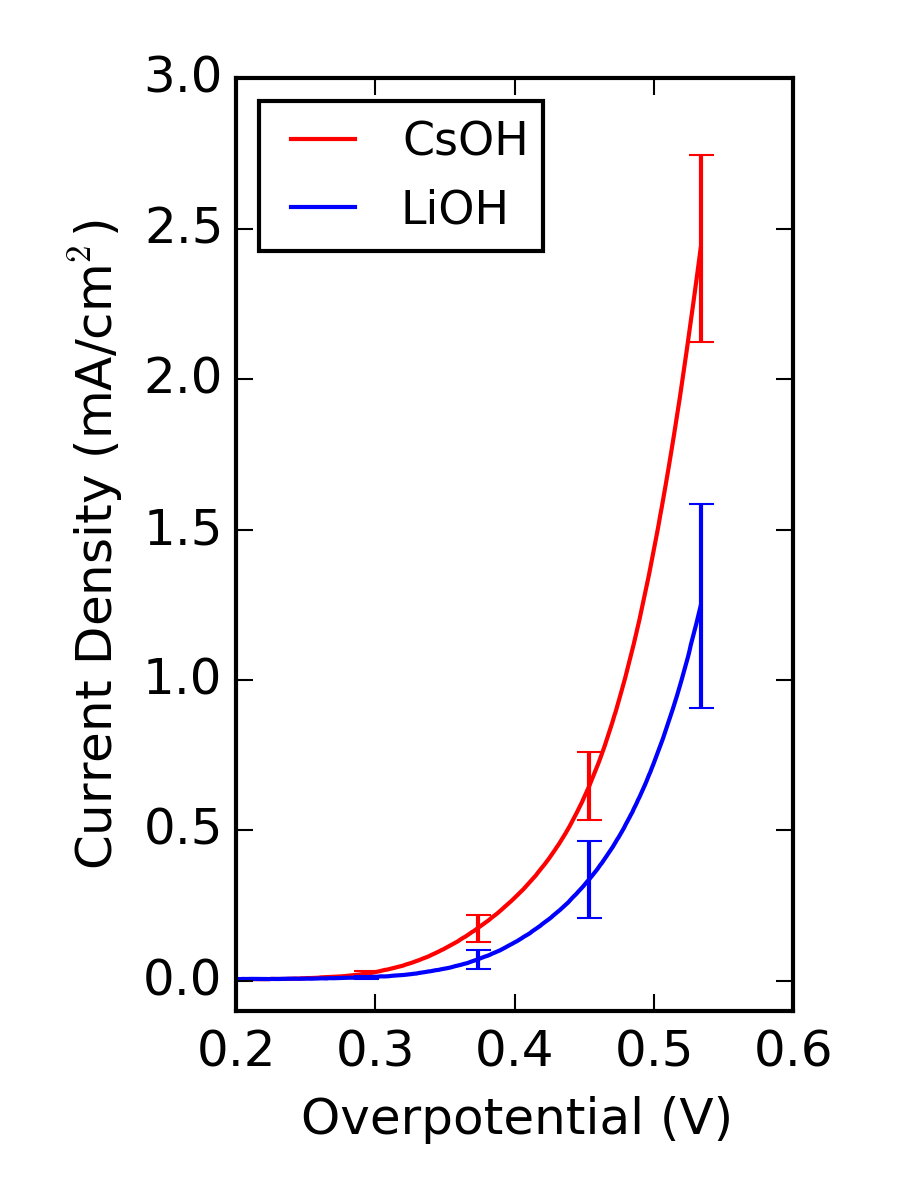
\includegraphics[width=3in]{./images/figures-supp-info/IvsV-Li-Cs-pure-10-08.png}
\caption{\label{fig-s1}LSV in purified CsOH (red) and LiOH (blue). Potential was swept at 1 mV/s. Error bars represent one standard deviation from mean current density at each corresponding potential.}
\end{figure}

\subsection{LSV with Electrolyte Switching in Purified NaOH and KOH}
\label{sec-2-2}
Figure \ref{fig-s2} shows the results of LSV while switching the electrolyte between purified NaOH (0.1 M) and KOH (0.1 M). Based on Figure \ref{fig-s2}, a relatively small cation effect was observed in purified NaOH and KOH. KOH promoted slightly higher OER current densities than NaOH. The differences in catalytic performance between purified CsOH and LiOH were smaller than the differences in catalytic performance observed in Figure \ref{fig-s1}.

\begin{figure}[h]
\centering
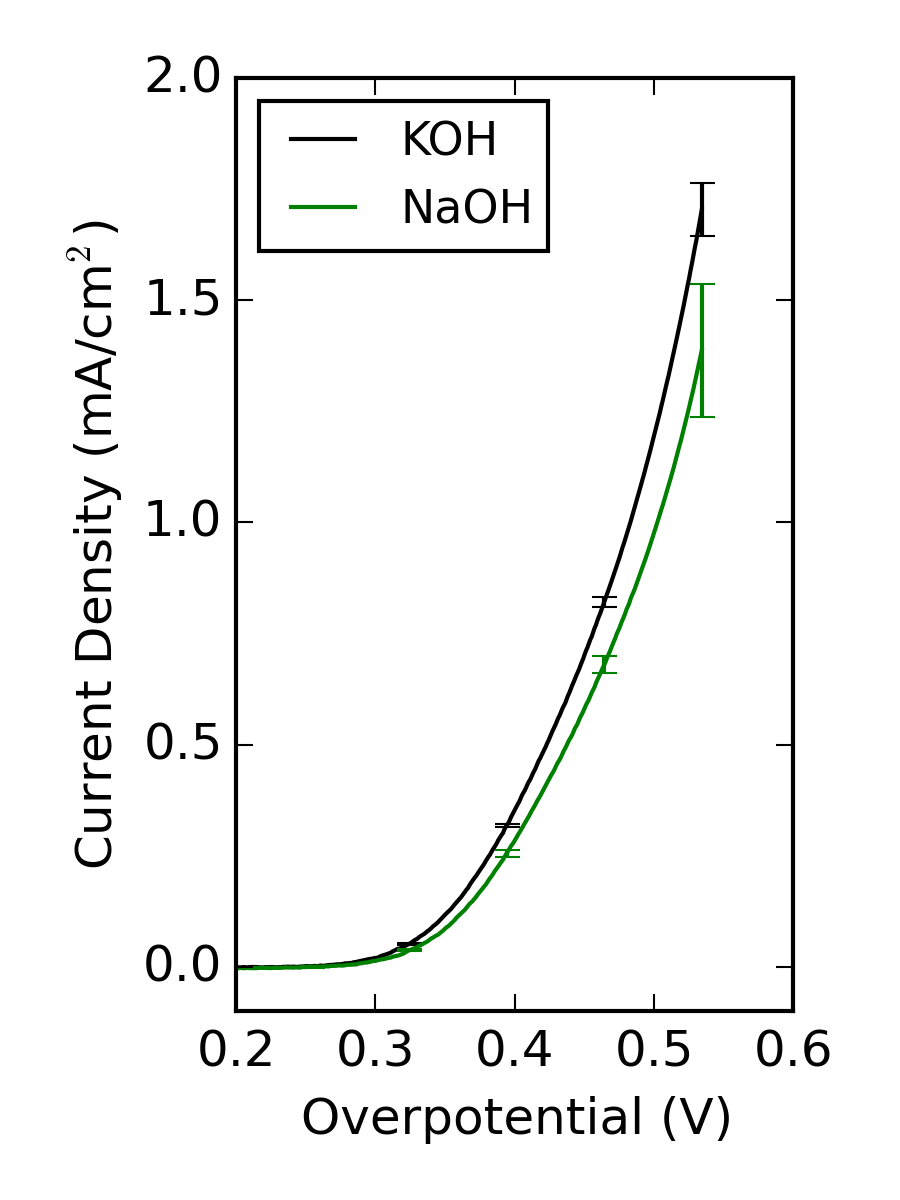
\includegraphics[width=3in]{./images/figures-supp-info/IvsV-Na-K-pure-01-16-15.png}
\caption{\label{fig-s2}LSV in purified KOH (black) and NaOH (green). Potential was swept at 1 mV/s. Error bars represent one standard deviation from mean current density at each corresponding potential.}
\end{figure}

\subsection{LSV with Electrolyte Switching in Fe-saturated LiOH and CsOH}
\label{sec-2-3}
Figure \ref{fig-s3} shows the results of LSV while switching the electrolyte between Fe-saturated LiOH (0.1 M) and CsOH (0.1 M). A cation effect on catalytic performance was observed in Fe-saturated electrolyte. Based on Figure \ref{fig-s3}, Fe-saturated CsOH promoted OER current densities that were $\approx$50 \% higher than OER current densities promoted by Fe-saturated LiOH.
\begin{figure}[h]
\centering
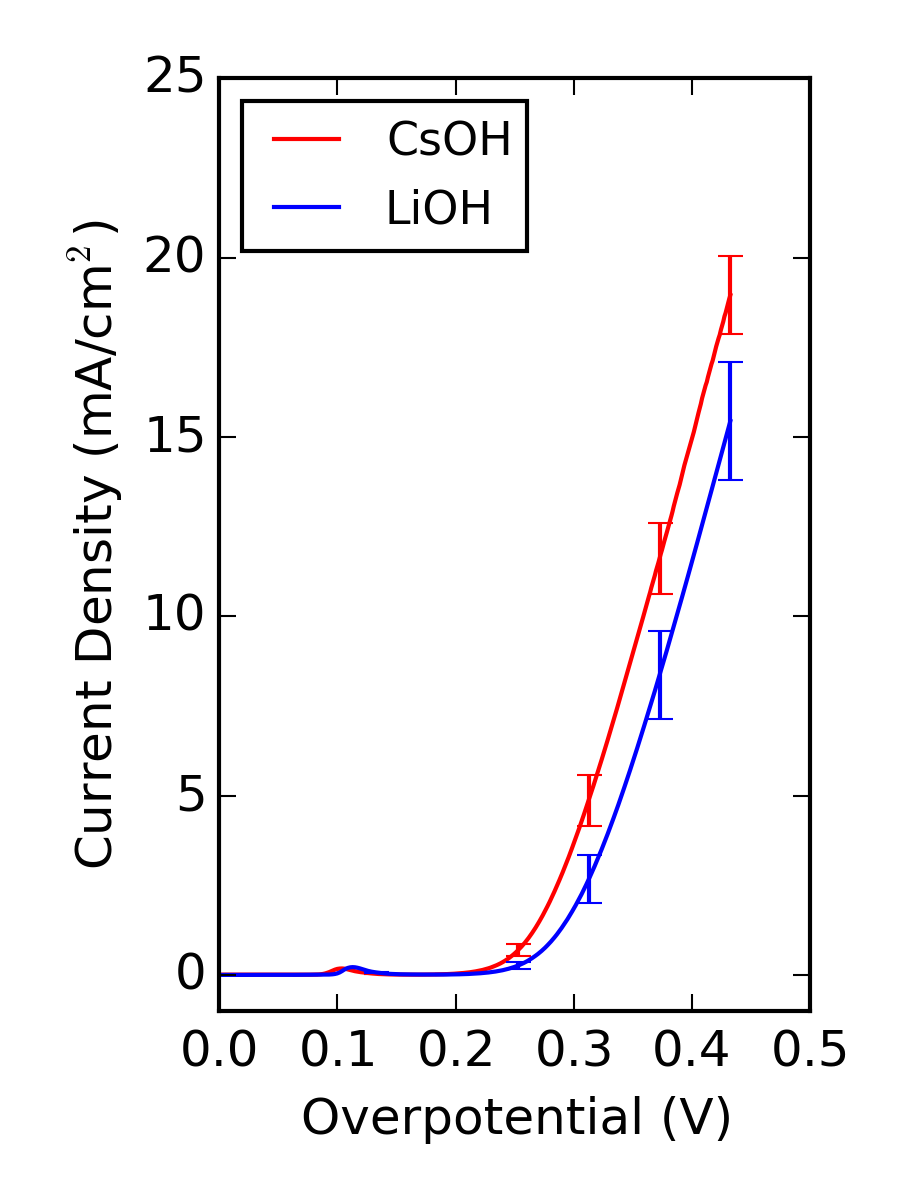
\includegraphics[width=3in]{./images/figures-supp-info/IvsV-Li-Cs-iron-11-21.png}
\caption{\label{fig-s3}LSV in purified CsOH (red) and LiOH (blue). Potential was swept at 1 mV/s. Error bars represent one standard deviation from mean current density at each corresponding potential.}
\end{figure}

\subsection{LSV with Electrolyte Switching in Fe-saturated NaOH and KOH}
\label{sec-2-4}
Figure \ref{fig-s4} shows the results of LSV while switching the electrolyte between Fe-saturated NaOH (0.1 M) and KOH (0.1 M). A cation effect on catalyst performance was not observed between Fe-saturated NaOH and KOH. Most of the NaOH current densities (green) overlapped with the KOH current densities (black). Current densities likely diverged at overpotentials above $\approx$0.35 V due to differences in oxygen bubble coverage on the working electrode surface, which would impede the flow of current.

\begin{figure}[h]
\centering
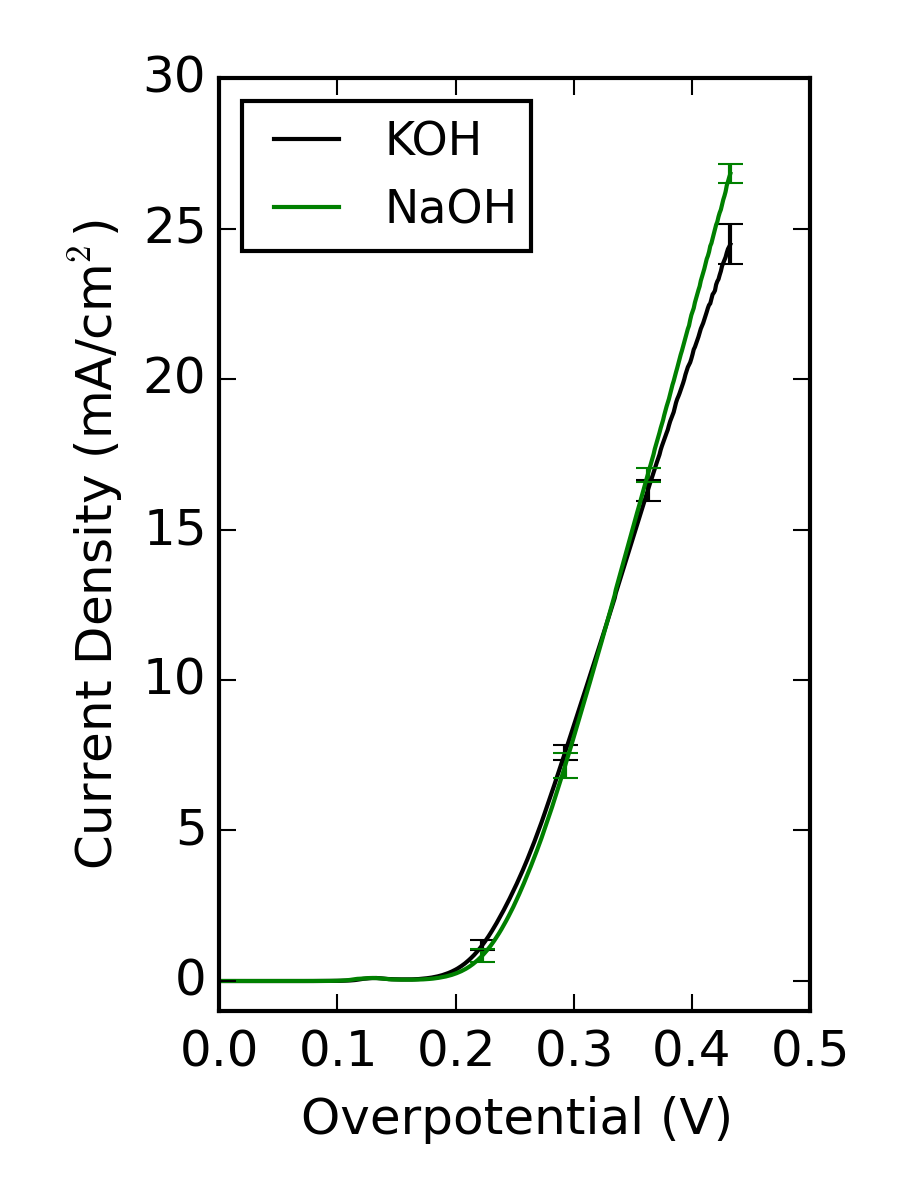
\includegraphics[width=3in]{./images/figures-supp-info/IvsV-Na-K-iron-01-19.png}
\caption{\label{fig-s4}LSV in Fe-saturated NaOH (green) and KOH (black). Potential was swept at 1 mV/s. Error bars represent one standard deviation from mean current density at each corresponding potential.}
\end{figure}

\subsection{LSV during Raman Spectroscopy in Purified LiOH and CsOH}
\label{sec-2-5}
Figure \ref{fig-s5} shows the results of LSV performed during Raman spectroscopy in purified LiOH (0.1 M) and CsOH (0.1 M). The corresponding Raman spectra are in Figure 3 (main text). Based on Figure \ref{fig-s5}, purified CsOH promoted OER current densities that were $\approx$50\% higher than OER current densities promoted by purified LiOH. Spectra were collected at overpotentials of 240, 340, and 440 mV.

\begin{figure}[h]
\centering
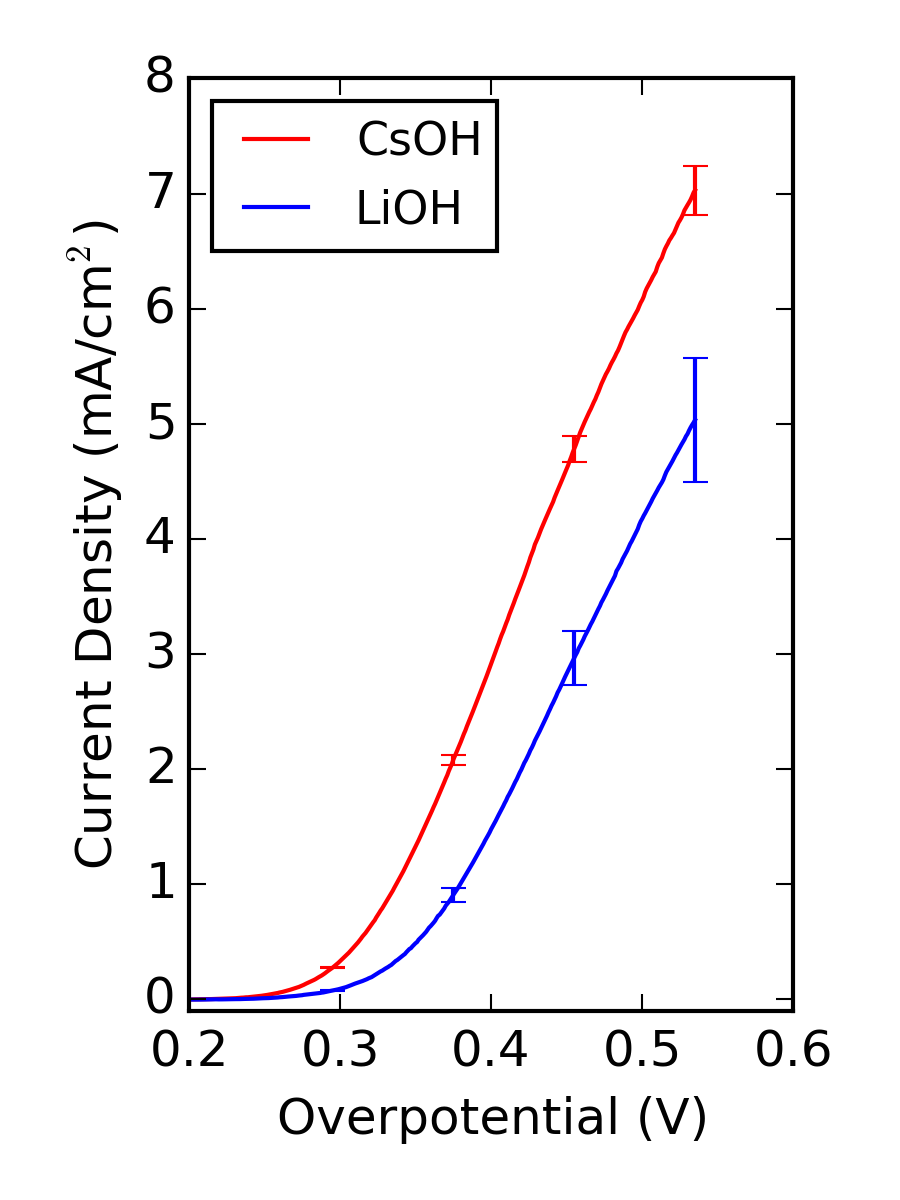
\includegraphics[width=3in]{./images/figures-supp-info/IvsV-Raman-Li-Cs-pure-10-31.png}
\caption{\label{fig-s5}LSV during Raman spectroscopy in Fe-saturated CsOH (red) and LiOH (blue). Potential was swept at 1 mV/s. Spectra were collected at 240, 340, and 440 mV. Error bars represent one standard deviation from mean current density at each corresponding potential.}
\end{figure}

\subsection{LSV during Raman Spectroscopy in Fe-saturated LiOH and CsOH}
\label{sec-2-6}
Figure \ref{fig-s6} shows the results of LSV performed during Raman spectroscopy in Fe-saturated LiOH (0.1 M) and CsOH (0.1 M). The corresponding Raman spectra are in Figure 4 (main text). Based on Figure \ref{fig-s6}, Fe-saturated CsOH promoted OER current densities that were $\approx$50\% higher than OER current densities promoted by Fe-saturated LiOH. Spectra were collected at overpotentials of 240, 340, and 440 mV.

\begin{figure}[H]
\centering
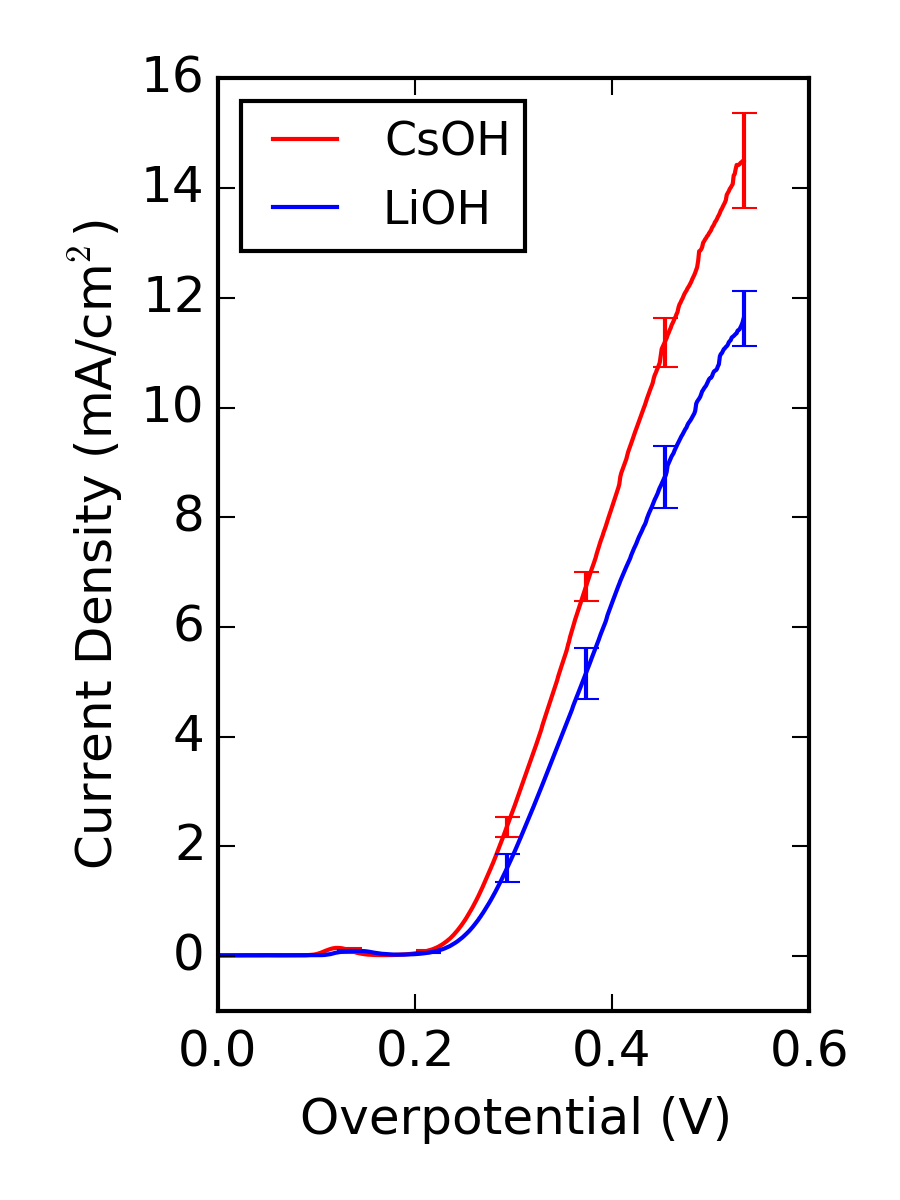
\includegraphics[width=3in]{./images/figures-supp-info/IvsV-Raman-Li-Cs-iron-11-19.png}
\caption{\label{fig-s6}LSV during Raman spectroscopy in Fe-saturated CsOH (red) and LiOH (blue). Potential was swept at 1 mV/s. Spectra were collected at 240, 340, and 440 mV. Error bars represent one standard deviation from mean current density at each corresponding potential.}
\end{figure}

\subsection{Tafel Analysis}
\label{sec-2-7}
Table \ref{tab:s1} shows the results of a Tafel analysis performed on LSV curves in purified and Fe-saturated LiOH, NaOH, KOH, and CsOH. Error represents one standard deviation from mean Tafel slope.

\begin{table}[H]
\caption{\label{tab:s1}Average Tafel slope (mV/decade) in purified and Fe-saturated LiOH, NaOH, KOH, and CsOH. Error represents one standard deviation from mean Tafel slope.}
\centering
\begin{tabular}{| c | c |}
\hline
\textbf{Electrolyte} & \textbf{Tafel slope (mv/decade)}\\
\hline
LiOH, purified & 56.95 \textpm \enspace 6.49\\
\hline
NaOH, purified & 61.66 \textpm \enspace 4.77\\
\hline
KOH, purified & 61.45 \textpm \enspace 2.70\\
\hline
CsOH, purified & 58.22 \textpm \enspace 8.74\\
\hline
LiOH, Fe-saturated & 21.39 \textpm \enspace 0.75\\
\hline
NaOH, Fe-saturated & 18.75 \textpm \enspace 1.09\\
\hline
KOH, Fe-saturated & 19.73 \textpm \enspace 0.96\\
\hline
CsOH, Fe-saturated & 21.57 \textpm \enspace 0.14\\
\hline
\end{tabular}
\end{table}

There was not a statistically significant difference between purified LiOH, NaOH, KOH, or CsOH; all Tafel slopes were $\approx$60 mV/decade. In addition, there was not a statistically significant difference between Fe-saturated LiOH, NaOH, KOH, or CsOH; all Tafel slopes were $\approx$20 mV/decade. Although these results do not provide much insight into the subtle differences in the current regimes, they clearly show that Fe had a significant effect on catalytic performance.

\section{Raman Spectra of Ni(OH)$_{\text{2}}$}
\label{sec-3}
Figure \ref{fig-s7} shows Raman spectra collected on Ni(OH)$_{\text{2}}$ thin films at 300 mV (vs. Hg/HgO). These were same thin films used for the LSV/Raman spectroscopy experiments described in the main body of this report, except the films were in a reduced state (i.e. Ni(OH)$_{\text{2}}$) and OER was not occurring. Figure \ref{fig-s7} shows no sharp Raman peaks at $\approx$480 cm$^{\text{-1}}$ and $\approx$560 cm$^{\text{-1}}$ (as in Figures 3 and 4, main text), indicating that the film was Ni(OH)$_{\text{2}}$ at an overpotential of 300 mV.

\begin{figure}[h]
\centering
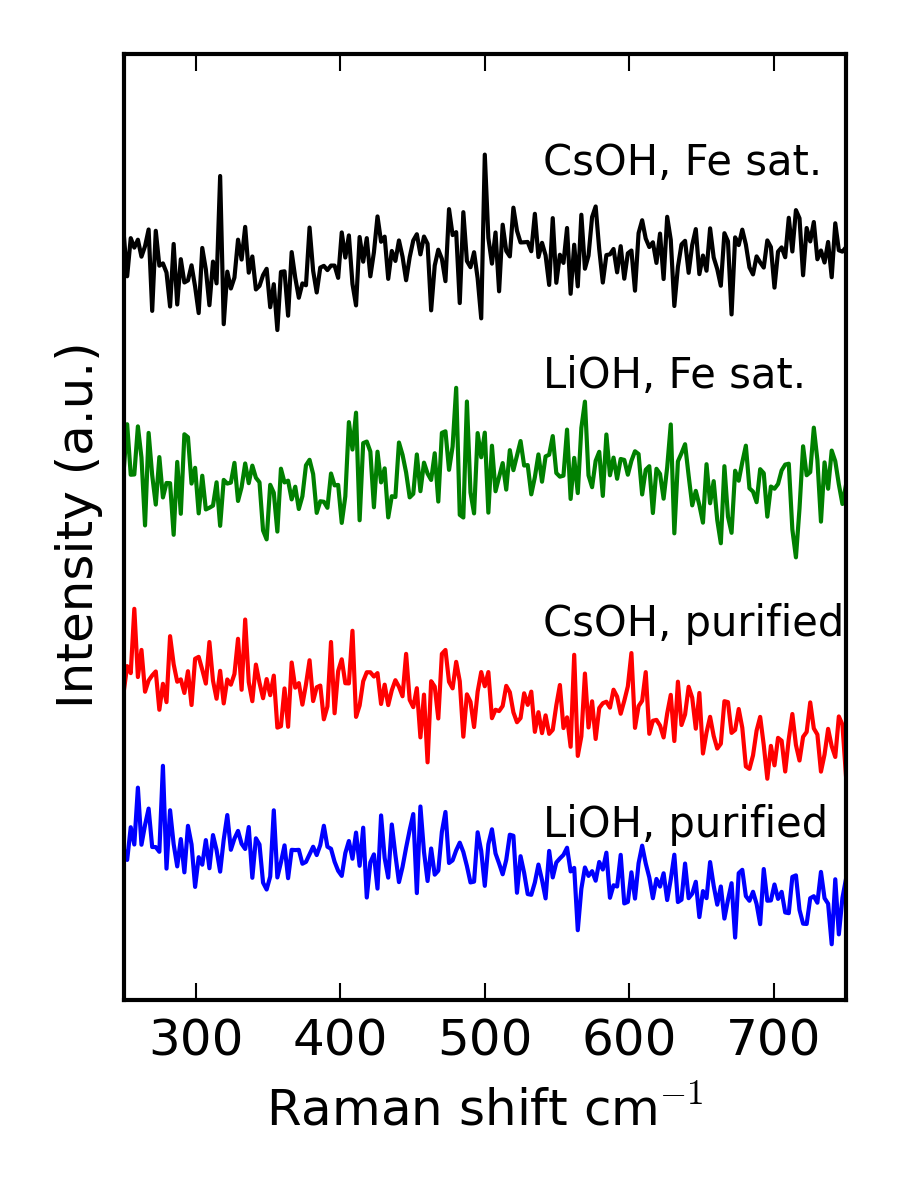
\includegraphics[width=3in]{./images/figures-supp-info/raman-nioh2-pure-iron.png}
\caption{\label{fig-s7}Raman spectra of Ni(OH)$_{\text{2}}$ at 300 mV (vs. Hg/HgO) in Fe-saturated CsOH (black), Fe-saturated LiOH (green), purified CsOH (red), and purified LiOH (blue).}
\end{figure}

\section{Results of Fitting Gaussian Functions to Raman spectra}
\label{sec-4}
Below is an expression with four Gaussian terms that was fit to Raman spectra for NiOOH.

$$y = \sum_{1}^{4} A_{n} exp\left (\frac{(x-B_{n})^{2}}{2C_{n}^{2}}\right )$$

A$_{\text{n}}$ is amplitude (a.u.), B$_{\text{n}}$ is mean peak position (cm$^{\text{-1}}$), C$_{\text{n}}$ is standard deviation (cm$^{\text{-1}}$), x is Raman shift (cm$^{\text{-1}}$), and y is Raman signal (a.u.). Subscripts n=1 and n=2 correspond to the two Gaussian curves fit to the peak at $\approx$480cm$^{\text{-1}}$ and subscripts n=3 and n=4 correspond to the two Gaussian curves fit to the peak at $\approx$560 cm$^{\text{-1}}$.

Below are initial guess, fitted, and calculated output parameters for fittings performed on all NiOOH Raman spectra for this manuscript. To call the curve fitting funtion, the following was typed (default settings included): dgaus2p(filename, cntr=(470, 560), amp1=(20, 20), amp2=(20, 20), std1=(10, 5), std2=(10, 5), datarange=None, output=False, step=4). Aside from the file name and step number, only default parameters that needed to be adjusted were included in the following code blocks. Python code for the "dgaus2p" function can be found in the Appendix below.

\subsection{Purified Electrolyte}
\label{sec-4-1}
\begin{enumerate}
\item LiOH
\label{sec-4-1-0-1}
\begin{enumerate}
\item Trial 1
\label{sec-4-1-0-1-1}
\begin{enumerate}
\item 600 mV
\label{sec-4-1-0-1-1-1}
\begin{minted}[frame=lines,fontsize=\scriptsize,linenos]{python}
from ramantools import dgaus2p

dgaus2p('./data/raman-spectra-for-fitting/purified/Ni-Li-pure-1-600mV.txt',
        cntr=(480, 560),
        amp1=(12, 12),
        amp2=(5, 5),
        output=True,
        step=4)

# Print initial guess, fitted, and calculated output parameters
with open('./data/raman-spectra-for-fitting/purified/Ni-Li-pure-1-600mV.fit', 'r') as f:
    print f.read()
\end{minted}

\begin{verbatim}
Initial guess parameters:
=========================
                      Peak 1, Peak 2
Peak center =         480.0, 560.00
Amplitude fit 1 =     12.0, 12.00
Amplitude fit 2 =     5.0, 5.00
Standard dev. fit 1 = 10.0, 5.0
Standard dev. fit 2 = 10.0, 5.0

Baseline parameters:
=========================
Slope =               -0.01
Intercept =           11.15

Fitted parameters:
=========================
                      Peak 1, Peak 2
Peak center =         479.80, 561.93
Amplitude fit 1 =     3.24, 19.47
Amplitude fit 2 =     5.94, 5.24
Standard dev. fit 1 = 31.33, 9.02
Standard dev. fit 2 = 29.63, 7.35

Calculation output:
========================
Mean peak 1 =         479.8 $\pm$ 0.23
Mean peak 2 =         561.9 $\pm$ 0.67
Height peak 1 =       28.9 $\pm$ 0.35
Height peak 2 =       16.5 $\pm$ 0.38
Area peak 1 =         982.4
Area peak 2 =         759.8
\end{verbatim}

\item 700 mV
\label{sec-4-1-0-1-1-2}
\begin{minted}[frame=lines,fontsize=\scriptsize,linenos]{python}
from ramantools import dgaus2p

dgaus2p('./data/raman-spectra-for-fitting/purified/Ni-Li-pure-1-700mV.txt',
        cntr=(480, 560),
        amp1=(12, 12),
        amp2=(5, 5),
        output=True,
        step=4)

# Print initial guess, fitted, and calculated output parameters
with open('./data/raman-spectra-for-fitting/purified/Ni-Li-pure-1-700mV.fit', 'r') as f:
    print f.read()
\end{minted}

\begin{verbatim}
Initial guess parameters:
=========================
                      Peak 1, Peak 2
Peak center =         480.0, 560.00
Amplitude fit 1 =     12.0, 12.00
Amplitude fit 2 =     5.0, 5.00
Standard dev. fit 1 = 10.0, 5.0
Standard dev. fit 2 = 10.0, 5.0

Baseline parameters:
=========================
Slope =               -0.01
Intercept =           10.27

Fitted parameters:
=========================
                      Peak 1, Peak 2
Peak center =         480.87, 561.94
Amplitude fit 1 =     5.30, 17.46
Amplitude fit 2 =     6.28, 6.96
Standard dev. fit 1 = 23.36, 7.78
Standard dev. fit 2 = 31.53, 6.82

Calculation output:
========================
Mean peak 1 =         480.9 $\pm$ 0.23
Mean peak 2 =         561.9 $\pm$ 0.53
Height peak 1 =       28.6 $\pm$ 0.38
Height peak 2 =       18.3 $\pm$ 0.37
Area peak 1 =         920.1
Area peak 2 =         869.3
\end{verbatim}

\item 800 mV
\label{sec-4-1-0-1-1-3}
\begin{minted}[frame=lines,fontsize=\scriptsize,linenos]{python}
from ramantools import dgaus2p

dgaus2p('./data/raman-spectra-for-fitting/purified/Ni-Li-pure-1-800mV.txt',
        cntr=(480, 560),
        amp1=(18, 18),
        amp2=(8, 8),
        output=True,
        step=4)

# Print initial guess, fitted, and calculated output parameters
with open('./data/raman-spectra-for-fitting/purified/Ni-Li-pure-1-800mV.fit', 'r') as f:
    print f.read()
\end{minted}

\begin{verbatim}
Initial guess parameters:
=========================
                      Peak 1, Peak 2
Peak center =         480.0, 560.00
Amplitude fit 1 =     18.0, 18.00
Amplitude fit 2 =     8.0, 8.00
Standard dev. fit 1 = 10.0, 5.0
Standard dev. fit 2 = 10.0, 5.0

Baseline parameters:
=========================
Slope =               -0.01
Intercept =           12.52

Fitted parameters:
=========================
                      Peak 1, Peak 2
Peak center =         480.96, 559.90
Amplitude fit 1 =     11.35, 15.80
Amplitude fit 2 =     8.16, 8.55
Standard dev. fit 1 = 17.09, 7.00
Standard dev. fit 2 = 30.13, 6.84

Calculation output:
========================
Mean peak 1 =         481.0 $\pm$ 0.21
Mean peak 2 =         559.9 $\pm$ 0.43
Height peak 1 =       34.6 $\pm$ 0.42
Height peak 2 =       23.3 $\pm$ 0.37
Area peak 1 =         1079.8
Area peak 2 =         1078.5
\end{verbatim}
\end{enumerate}

\item Trial 2
\label{sec-4-1-0-1-2}
\begin{enumerate}
\item 600 mV
\label{sec-4-1-0-1-2-1}
\begin{minted}[frame=lines,fontsize=\scriptsize,linenos]{python}
from ramantools import dgaus2p

dgaus2p('./data/raman-spectra-for-fitting/purified/Ni-Li-pure-2-600mV.txt',
        cntr=(480, 560),
        amp1=(15, 15),
        amp2=(8, 8),
        output=True,
        step=4)

# Print file containing input, fitted, and output parameters
with open('./data/raman-spectra-for-fitting/purified/Ni-Li-pure-2-600mV.fit', 'r') as f:
    print f.read()
\end{minted}

\begin{verbatim}
Initial guess parameters:
=========================
                      Peak 1, Peak 2
Peak center =         480.0, 560.00
Amplitude fit 1 =     15.0, 15.00
Amplitude fit 2 =     8.0, 8.00
Standard dev. fit 1 = 10.0, 5.0
Standard dev. fit 2 = 10.0, 5.0

Baseline parameters:
=========================
Slope =               -0.01
Intercept =           11.61

Fitted parameters:
=========================
                      Peak 1, Peak 2
Peak center =         480.69, 562.66
Amplitude fit 1 =     3.47, 17.77
Amplitude fit 2 =     6.25, 5.66
Standard dev. fit 1 = 30.74, 8.91
Standard dev. fit 2 = 28.11, 7.15

Calculation output:
========================
Mean peak 1 =         480.7 $\pm$ 0.26
Mean peak 2 =         562.7 $\pm$ 0.61
Height peak 1 =       28.3 $\pm$ 0.35
Height peak 2 =       18.1 $\pm$ 0.39
Area peak 1 =         939.7
Area peak 2 =         766.3
\end{verbatim}

\item 700 mV
\label{sec-4-1-0-1-2-2}
\begin{minted}[frame=lines,fontsize=\scriptsize,linenos]{python}
from ramantools import dgaus2p

dgaus2p('./data/raman-spectra-for-fitting/purified/Ni-Li-pure-2-700mV.txt',
        cntr=(480, 560),
        amp1=(12, 12),
        amp2=(10, 10),
        output=True,
        step=4)

# Print initial guess, fitted, and calculated output parameters
with open('./data/raman-spectra-for-fitting/purified/Ni-Li-pure-2-700mV.fit', 'r') as f:
    print f.read()
\end{minted}

\begin{verbatim}
Initial guess parameters:
=========================
                      Peak 1, Peak 2
Peak center =         480.0, 560.00
Amplitude fit 1 =     12.0, 12.00
Amplitude fit 2 =     10.0, 10.00
Standard dev. fit 1 = 10.0, 5.0
Standard dev. fit 2 = 10.0, 5.0

Baseline parameters:
=========================
Slope =               -0.01
Intercept =           12.84

Fitted parameters:
=========================
                      Peak 1, Peak 2
Peak center =         480.61, 562.13
Amplitude fit 1 =     9.47, 16.34
Amplitude fit 2 =     8.06, 7.08
Standard dev. fit 1 = 18.32, 7.09
Standard dev. fit 2 = 29.43, 6.88

Calculation output:
========================
Mean peak 1 =         480.6 $\pm$ 0.21
Mean peak 2 =         562.1 $\pm$ 0.49
Height peak 1 =       33.0 $\pm$ 0.40
Height peak 2 =       21.4 $\pm$ 0.36
Area peak 1 =         1025.5
Area peak 2 =         1012.7
\end{verbatim}

\item 800 mV
\label{sec-4-1-0-1-2-3}
\begin{minted}[frame=lines,fontsize=\scriptsize,linenos]{python}
from ramantools import dgaus2p

dgaus2p('./data/raman-spectra-for-fitting/purified/Ni-Li-pure-2-800mV.txt',
        cntr=(480, 560),
        amp1=(15, 15),
        amp2=(10, 10),
        output=True,
        step=4)

# Print initial guess, fitted, and calculated output parameters
with open('./data/raman-spectra-for-fitting/purified/Ni-Li-pure-2-800mV.fit', 'r') as f:
    print f.read()
\end{minted}

\begin{verbatim}
Initial guess parameters:
=========================
                      Peak 1, Peak 2
Peak center =         480.0, 560.00
Amplitude fit 1 =     15.0, 15.00
Amplitude fit 2 =     10.0, 10.00
Standard dev. fit 1 = 10.0, 5.0
Standard dev. fit 2 = 10.0, 5.0

Baseline parameters:
=========================
Slope =               -0.01
Intercept =           12.83

Fitted parameters:
=========================
                      Peak 1, Peak 2
Peak center =         481.12, 562.23
Amplitude fit 1 =     5.23, 22.32
Amplitude fit 2 =     8.94, 8.21
Standard dev. fit 1 = 28.56, 8.52
Standard dev. fit 2 = 30.69, 5.68

Calculation output:
========================
Mean peak 1 =         481.1 $\pm$ 0.21
Mean peak 2 =         562.2 $\pm$ 0.43
Height peak 1 =       35.1 $\pm$ 0.39
Height peak 2 =       23.8 $\pm$ 0.46
Area peak 1 =         1203.4
Area peak 2 =         1137.4
\end{verbatim}
\end{enumerate}

\item Trial 3
\label{sec-4-1-0-1-3}
\begin{enumerate}
\item 600 mV
\label{sec-4-1-0-1-3-1}
\begin{minted}[frame=lines,fontsize=\scriptsize,linenos]{python}
from ramantools import dgaus2p

dgaus2p('./data/raman-spectra-for-fitting/purified/Ni-Li-pure-3-600mV.txt',
        cntr=(480, 560),
        amp1=(20, 20),
        amp2=(10, 10),
        output=True,
        step=4)

# Print file containing input, fitted, and output parameters
with open('./data/raman-spectra-for-fitting/purified/Ni-Li-pure-3-600mV.fit', 'r') as f:
    print f.read()
\end{minted}

\begin{verbatim}
Initial guess parameters:
=========================
                      Peak 1, Peak 2
Peak center =         480.0, 560.00
Amplitude fit 1 =     20.0, 20.00
Amplitude fit 2 =     10.0, 10.00
Standard dev. fit 1 = 10.0, 5.0
Standard dev. fit 2 = 10.0, 5.0

Baseline parameters:
=========================
Slope =               -0.02
Intercept =           20.39

Fitted parameters:
=========================
                      Peak 1, Peak 2
Peak center =         480.76, 561.57
Amplitude fit 1 =     6.48, 29.63
Amplitude fit 2 =     11.85, 9.42
Standard dev. fit 1 = 27.52, 9.17
Standard dev. fit 2 = 28.01, 6.83

Calculation output:
========================
Mean peak 1 =         480.8 $\pm$ 0.18
Mean peak 2 =         561.6 $\pm$ 0.40
Height peak 1 =       49.0 $\pm$ 0.41
Height peak 2 =       32.9 $\pm$ 0.45
Area peak 1 =         1594.5
Area peak 2 =         1404.9
\end{verbatim}

\item 700 mV
\label{sec-4-1-0-1-3-2}
\begin{minted}[frame=lines,fontsize=\scriptsize,linenos]{python}
from ramantools import dgaus2p

dgaus2p('./data/raman-spectra-for-fitting/purified/Ni-Li-pure-3-700mV.txt',
        cntr=(480, 560),
        amp1=(25, 25),
        amp2=(15, 15),
        output=True,
        step=4)

# Print initial guess, fitted, and calculated output parameters
with open('./data/raman-spectra-for-fitting/purified/Ni-Li-pure-3-700mV.fit', 'r') as f:
    print f.read()
\end{minted}

\begin{verbatim}
Initial guess parameters:
=========================
                      Peak 1, Peak 2
Peak center =         480.0, 560.00
Amplitude fit 1 =     25.0, 25.00
Amplitude fit 2 =     15.0, 15.00
Standard dev. fit 1 = 10.0, 5.0
Standard dev. fit 2 = 10.0, 5.0

Baseline parameters:
=========================
Slope =               -0.01
Intercept =           20.07

Fitted parameters:
=========================
                      Peak 1, Peak 2
Peak center =         481.28, 561.82
Amplitude fit 1 =     7.69, 32.53
Amplitude fit 2 =     11.77, 12.42
Standard dev. fit 1 = 27.54, 9.09
Standard dev. fit 2 = 31.39, 7.37

Calculation output:
========================
Mean peak 1 =         481.3 $\pm$ 0.17
Mean peak 2 =         561.8 $\pm$ 0.37
Height peak 1 =       53.2 $\pm$ 0.44
Height peak 2 =       36.0 $\pm$ 0.46
Area peak 1 =         1798.8
Area peak 2 =         1632.5
\end{verbatim}

\item 800 mV
\label{sec-4-1-0-1-3-3}
\begin{minted}[frame=lines,fontsize=\scriptsize,linenos]{python}
from ramantools import dgaus2p

dgaus2p('./data/raman-spectra-for-fitting/purified/Ni-Li-pure-3-800mV.txt',
        cntr=(480, 560),
        amp1=(20, 20),
        amp2=(15, 15),
        output=True,
        step=4)

# Print initial guess, fitted, and calculated output parameters
with open('./data/raman-spectra-for-fitting/purified/Ni-Li-pure-3-800mV.fit', 'r') as f:
    print f.read()
\end{minted}

\begin{verbatim}
Initial guess parameters:
=========================
                      Peak 1, Peak 2
Peak center =         480.0, 560.00
Amplitude fit 1 =     20.0, 20.00
Amplitude fit 2 =     15.0, 15.00
Standard dev. fit 1 = 10.0, 5.0
Standard dev. fit 2 = 10.0, 5.0

Baseline parameters:
=========================
Slope =               -0.01
Intercept =           18.86

Fitted parameters:
=========================
                      Peak 1, Peak 2
Peak center =         481.70, 561.30
Amplitude fit 1 =     6.45, 36.69
Amplitude fit 2 =     12.66, 14.57
Standard dev. fit 1 = 33.81, 9.49
Standard dev. fit 2 = 30.84, 6.88

Calculation output:
========================
Mean peak 1 =         481.7 $\pm$ 0.16
Mean peak 2 =         561.3 $\pm$ 0.31
Height peak 1 =       55.5 $\pm$ 0.43
Height peak 2 =       38.5 $\pm$ 0.48
Area peak 1 =         2006.8
Area peak 2 =         1738.6
\end{verbatim}
\end{enumerate}
\end{enumerate}

\item CsOH
\label{sec-4-1-0-2}
\begin{enumerate}
\item Trial 1
\label{sec-4-1-0-2-1}
\begin{enumerate}
\item 600 mV
\label{sec-4-1-0-2-1-1}
\begin{minted}[frame=lines,fontsize=\scriptsize,linenos]{python}
from ramantools import dgaus2p

dgaus2p('./data/raman-spectra-for-fitting/purified/Ni-Cs-pure-1-600mV.txt',
        cntr=(480, 560),
        amp1=(20, 20),
        amp2=(15, 15),
        output=True,
        step=4)

# Print initial guess, fitted, and calculated output parameters
with open('./data/raman-spectra-for-fitting/purified/Ni-Cs-pure-1-600mV.fit', 'r') as f:
    print f.read()
\end{minted}

\begin{verbatim}
Initial guess parameters:
=========================
                      Peak 1, Peak 2
Peak center =         480.0, 560.00
Amplitude fit 1 =     20.0, 20.00
Amplitude fit 2 =     15.0, 15.00
Standard dev. fit 1 = 10.0, 5.0
Standard dev. fit 2 = 10.0, 5.0

Baseline parameters:
=========================
Slope =               -0.02
Intercept =           21.12

Fitted parameters:
=========================
                      Peak 1, Peak 2
Peak center =         479.26, 557.07
Amplitude fit 1 =     16.45, 27.02
Amplitude fit 2 =     11.32, 14.54
Standard dev. fit 1 = 18.12, 7.04
Standard dev. fit 2 = 28.89, 6.63

Calculation output:
========================
Mean peak 1 =         479.3 $\pm$ 0.15
Mean peak 2 =         557.1 $\pm$ 0.30
Height peak 1 =       57.4 $\pm$ 0.48
Height peak 2 =       38.6 $\pm$ 0.44
Area peak 1 =         1731.1
Area peak 2 =         1500.6
\end{verbatim}

\item 700 mV
\label{sec-4-1-0-2-1-2}
\begin{minted}[frame=lines,fontsize=\scriptsize,linenos]{python}
from ramantools import dgaus2p

dgaus2p('./data/raman-spectra-for-fitting/purified/Ni-Cs-pure-1-700mV.txt',
        cntr=(480, 560),
        amp1=(25, 25),
        amp2=(15, 15),
        output=True,
        step=4)

# Print initial guess, fitted, and calculated output parameters
with open('./data/raman-spectra-for-fitting/purified/Ni-Cs-pure-1-700mV.fit', 'r') as f:
    print f.read()
\end{minted}

\begin{verbatim}
Initial guess parameters:
=========================
                      Peak 1, Peak 2
Peak center =         480.0, 560.00
Amplitude fit 1 =     25.0, 25.00
Amplitude fit 2 =     15.0, 15.00
Standard dev. fit 1 = 10.0, 5.0
Standard dev. fit 2 = 10.0, 5.0

Baseline parameters:
=========================
Slope =               -0.02
Intercept =           21.56

Fitted parameters:
=========================
                      Peak 1, Peak 2
Peak center =         479.99, 557.14
Amplitude fit 1 =     16.38, 28.07
Amplitude fit 2 =     10.40, 18.14
Standard dev. fit 1 = 18.11, 7.04
Standard dev. fit 2 = 34.48, 6.90

Calculation output:
========================
Mean peak 1 =         480.0 $\pm$ 0.15
Mean peak 2 =         557.1 $\pm$ 0.26
Height peak 1 =       58.1 $\pm$ 0.48
Height peak 2 =       40.9 $\pm$ 0.43
Area peak 1 =         1751.9
Area peak 2 =         1711.4
\end{verbatim}

\item 800 mV
\label{sec-4-1-0-2-1-3}
\begin{minted}[frame=lines,fontsize=\scriptsize,linenos]{python}
from ramantools import dgaus2p

dgaus2p('./data/raman-spectra-for-fitting/purified/Ni-Cs-pure-1-800mV.txt',
        cntr=(480, 560),
        amp1=(25, 25),
        amp2=(20, 20),
        output=True,
        step=4)

# Print initial guess, fitted, and calculated output parameters
with open('./data/raman-spectra-for-fitting/purified/Ni-Cs-pure-1-800mV.fit', 'r') as f:
    print f.read()
\end{minted}

\begin{verbatim}
Initial guess parameters:
=========================
                      Peak 1, Peak 2
Peak center =         480.0, 560.00
Amplitude fit 1 =     25.0, 25.00
Amplitude fit 2 =     20.0, 20.00
Standard dev. fit 1 = 10.0, 5.0
Standard dev. fit 2 = 10.0, 5.0

Baseline parameters:
=========================
Slope =               -0.02
Intercept =           24.25

Fitted parameters:
=========================
                      Peak 1, Peak 2
Peak center =         479.75, 555.99
Amplitude fit 1 =     23.84, 27.04
Amplitude fit 2 =     12.69, 19.81
Standard dev. fit 1 = 15.58, 5.65
Standard dev. fit 2 = 33.62, 6.40

Calculation output:
========================
Mean peak 1 =         479.8 $\pm$ 0.13
Mean peak 2 =         556.0 $\pm$ 0.23
Height peak 1 =       66.6 $\pm$ 0.56
Height peak 2 =       46.9 $\pm$ 0.47
Area peak 1 =         1858.8
Area peak 2 =         1959.6
\end{verbatim}
\end{enumerate}

\item Trial 2
\label{sec-4-1-0-2-2}
\begin{enumerate}
\item 600 mV
\label{sec-4-1-0-2-2-1}
\begin{minted}[frame=lines,fontsize=\scriptsize,linenos]{python}
from ramantools import dgaus2p

dgaus2p('./data/raman-spectra-for-fitting/purified/Ni-Cs-pure-2-600mV.txt',
        cntr=(480, 560),
        amp1=(20, 20),
        amp2=(12, 12),
        output=True,
        step=4)

# Print initial guess, fitted, and calculated output parameters
with open('./data/raman-spectra-for-fitting/purified/Ni-Cs-pure-2-600mV.fit', 'r') as f:
    print f.read()
\end{minted}

\begin{verbatim}
Initial guess parameters:
=========================
                      Peak 1, Peak 2
Peak center =         480.0, 560.00
Amplitude fit 1 =     20.0, 20.00
Amplitude fit 2 =     12.0, 12.00
Standard dev. fit 1 = 10.0, 5.0
Standard dev. fit 2 = 10.0, 5.0

Baseline parameters:
=========================
Slope =               -0.01
Intercept =           13.45

Fitted parameters:
=========================
                      Peak 1, Peak 2
Peak center =         479.03, 556.93
Amplitude fit 1 =     18.44, 20.50
Amplitude fit 2 =     10.46, 12.56
Standard dev. fit 1 = 15.94, 5.84
Standard dev. fit 2 = 28.43, 6.01

Calculation output:
========================
Mean peak 1 =         479.0 $\pm$ 0.14
Mean peak 2 =         556.9 $\pm$ 0.29
Height peak 1 =       46.9 $\pm$ 0.46
Height peak 2 =       30.0 $\pm$ 0.41
Area peak 1 =         1466.6
Area peak 2 =         1321.5
\end{verbatim}

\item 700 mV
\label{sec-4-1-0-2-2-2}
\begin{minted}[frame=lines,fontsize=\scriptsize,linenos]{python}
from ramantools import dgaus2p

dgaus2p('./data/raman-spectra-for-fitting/purified/Ni-Cs-pure-2-700mV.txt',
        cntr=(480, 560),
        amp1=(20, 20),
        amp2=(13, 13),
        output=True,
        step=4)

# Print initial guess, fitted, and calculated output parameters
with open('./data/raman-spectra-for-fitting/purified/Ni-Cs-pure-2-700mV.fit', 'r') as f:
    print f.read()
\end{minted}

\begin{verbatim}
Initial guess parameters:
=========================
                      Peak 1, Peak 2
Peak center =         480.0, 560.00
Amplitude fit 1 =     20.0, 20.00
Amplitude fit 2 =     13.0, 13.00
Standard dev. fit 1 = 10.0, 5.0
Standard dev. fit 2 = 10.0, 5.0

Baseline parameters:
=========================
Slope =               -0.01
Intercept =           14.47

Fitted parameters:
=========================
                      Peak 1, Peak 2
Peak center =         479.42, 556.63
Amplitude fit 1 =     19.40, 20.75
Amplitude fit 2 =     10.76, 15.32
Standard dev. fit 1 = 14.97, 5.54
Standard dev. fit 2 = 29.82, 5.99

Calculation output:
========================
Mean peak 1 =         479.4 $\pm$ 0.14
Mean peak 2 =         556.6 $\pm$ 0.25
Height peak 1 =       49.0 $\pm$ 0.49
Height peak 2 =       34.0 $\pm$ 0.43
Area peak 1 =         1436.8
Area peak 2 =         1461.9
\end{verbatim}

\item 800 mV
\label{sec-4-1-0-2-2-3}
\begin{minted}[frame=lines,fontsize=\scriptsize,linenos]{python}
from ramantools import dgaus2p

dgaus2p('./data/raman-spectra-for-fitting/purified/Ni-Cs-pure-2-800mV.txt',
        cntr=(480, 560),
        amp1=(22, 22),
        amp2=(13, 13),
        output=True,
        step=4)

# Print initial guess, fitted, and calculated output parameters
with open('./data/raman-spectra-for-fitting/purified/Ni-Cs-pure-2-800mV.fit', 'r') as f:
    print f.read()
\end{minted}

\begin{verbatim}
Initial guess parameters:
=========================
                      Peak 1, Peak 2
Peak center =         480.0, 560.00
Amplitude fit 1 =     22.0, 22.00
Amplitude fit 2 =     13.0, 13.00
Standard dev. fit 1 = 10.0, 5.0
Standard dev. fit 2 = 10.0, 5.0

Baseline parameters:
=========================
Slope =               -0.01
Intercept =           15.21

Fitted parameters:
=========================
                      Peak 1, Peak 2
Peak center =         479.94, 557.19
Amplitude fit 1 =     11.88, 29.43
Amplitude fit 2 =     11.44, 15.79
Standard dev. fit 1 = 18.42, 7.95
Standard dev. fit 2 = 31.88, 6.28

Calculation output:
========================
Mean peak 1 =         479.9 $\pm$ 0.14
Mean peak 2 =         557.2 $\pm$ 0.27
Height peak 1 =       50.5 $\pm$ 0.44
Height peak 2 =       35.4 $\pm$ 0.43
Area peak 1 =         1604.8
Area peak 2 =         1643.5
\end{verbatim}
\end{enumerate}

\item Trial 3
\label{sec-4-1-0-2-3}
\begin{enumerate}
\item 600 mV
\label{sec-4-1-0-2-3-1}
\begin{minted}[frame=lines,fontsize=\scriptsize,linenos]{python}
from ramantools import dgaus2p

dgaus2p('./data/raman-spectra-for-fitting/purified/Ni-Cs-pure-3-600mV.txt',
        cntr=(480, 560),
        amp1=(15, 15),
        amp2=(8, 8),
        output=True,
        step=4)

# Print initial guess, fitted, and calculated output parameters
with open('./data/raman-spectra-for-fitting/purified/Ni-Cs-pure-3-600mV.fit', 'r') as f:
    print f.read()
\end{minted}

\begin{verbatim}
Initial guess parameters:
=========================
                      Peak 1, Peak 2
Peak center =         480.0, 560.00
Amplitude fit 1 =     15.0, 15.00
Amplitude fit 2 =     8.0, 8.00
Standard dev. fit 1 = 10.0, 5.0
Standard dev. fit 2 = 10.0, 5.0

Baseline parameters:
=========================
Slope =               -0.01
Intercept =           9.67

Fitted parameters:
=========================
                      Peak 1, Peak 2
Peak center =         478.33, 557.10
Amplitude fit 1 =     11.07, 14.10
Amplitude fit 2 =     5.99, 8.29
Standard dev. fit 1 = 15.73, 5.91
Standard dev. fit 2 = 31.73, 6.48

Calculation output:
========================
Mean peak 1 =         478.3 $\pm$ 0.21
Mean peak 2 =         557.1 $\pm$ 0.44
Height peak 1 =       30.9 $\pm$ 0.44
Height peak 2 =       19.4 $\pm$ 0.37
Area peak 1 =         912.3
Area peak 2 =         863.9
\end{verbatim}

\item 700 mV
\label{sec-4-1-0-2-3-2}
\begin{minted}[frame=lines,fontsize=\scriptsize,linenos]{python}
from ramantools import dgaus2p

dgaus2p('./data/raman-spectra-for-fitting/purified/Ni-Cs-pure-3-700mV.txt',
        cntr=(480, 560),
        amp1=(20, 20),
        amp2=(12, 12),
        output=True,
        step=4)

# Print initial guess, fitted, and calculated output parameters
with open('./data/raman-spectra-for-fitting/purified/Ni-Cs-pure-3-700mV.fit', 'r') as f:
    print f.read()
\end{minted}

\begin{verbatim}
Initial guess parameters:
=========================
                      Peak 1, Peak 2
Peak center =         480.0, 560.00
Amplitude fit 1 =     20.0, 20.00
Amplitude fit 2 =     12.0, 12.00
Standard dev. fit 1 = 10.0, 5.0
Standard dev. fit 2 = 10.0, 5.0

Baseline parameters:
=========================
Slope =               -0.01
Intercept =           12.83

Fitted parameters:
=========================
                      Peak 1, Peak 2
Peak center =         478.97, 557.14
Amplitude fit 1 =     16.18, 18.71
Amplitude fit 2 =     9.01, 11.93
Standard dev. fit 1 = 16.10, 5.74
Standard dev. fit 2 = 30.03, 6.17

Calculation output:
========================
Mean peak 1 =         479.0 $\pm$ 0.16
Mean peak 2 =         557.1 $\pm$ 0.30
Height peak 1 =       43.0 $\pm$ 0.45
Height peak 2 =       28.2 $\pm$ 0.39
Area peak 1 =         1304.4
Area peak 2 =         1219.4
\end{verbatim}

\item 800 mV
\label{sec-4-1-0-2-3-3}
\begin{minted}[frame=lines,fontsize=\scriptsize,linenos]{python}
from ramantools import dgaus2p

dgaus2p('./data/raman-spectra-for-fitting/purified/Ni-Cs-pure-3-800mV.txt',
        cntr=(480, 560),
        amp1=(20, 20),
        amp2=(13, 13),
        output=True,
        step=4)

# Print initial guess, fitted, and calculated output parameters
with open('./data/raman-spectra-for-fitting/purified/Ni-Cs-pure-3-800mV.fit', 'r') as f:
    print f.read()
\end{minted}

\begin{verbatim}
Initial guess parameters:
=========================
                      Peak 1, Peak 2
Peak center =         480.0, 560.00
Amplitude fit 1 =     20.0, 20.00
Amplitude fit 2 =     13.0, 13.00
Standard dev. fit 1 = 10.0, 5.0
Standard dev. fit 2 = 10.0, 5.0

Baseline parameters:
=========================
Slope =               -0.01
Intercept =           13.23

Fitted parameters:
=========================
                      Peak 1, Peak 2
Peak center =         479.64, 556.47
Amplitude fit 1 =     15.34, 19.03
Amplitude fit 2 =     9.32, 14.37
Standard dev. fit 1 = 15.69, 6.98
Standard dev. fit 2 = 32.33, 6.31

Calculation output:
========================
Mean peak 1 =         479.6 $\pm$ 0.17
Mean peak 2 =         556.5 $\pm$ 0.28
Height peak 1 =       42.4 $\pm$ 0.46
Height peak 2 =       30.9 $\pm$ 0.42
Area peak 1 =         1323.6
Area peak 2 =         1388.3
\end{verbatim}
\end{enumerate}
\end{enumerate}
\end{enumerate}

\subsection{Fe-saturated Electrolyte}
\label{sec-4-2}
\begin{enumerate}
\item LiOH
\label{sec-4-2-0-1}
\begin{enumerate}
\item Trial 1
\label{sec-4-2-0-1-1}
\begin{enumerate}
\item 600 mV
\label{sec-4-2-0-1-1-1}
\begin{minted}[frame=lines,fontsize=\scriptsize,linenos]{python}
from ramantools import dgaus2p

dgaus2p('./data/raman-spectra-for-fitting/iron-saturated/Ni-Li-Fe-1-600mV.txt',
        cntr=(480, 560),
        amp1=(12, 12),
        amp2=(10, 10),
        output=True,
        step=4)

# Print initial guess, fitted, and calculated output parameters
with open('./data/raman-spectra-for-fitting/iron-saturated/Ni-Li-Fe-1-600mV.fit', 'r') as f:
    print f.read()
\end{minted}

\begin{verbatim}
Initial guess parameters:
=========================
                      Peak 1, Peak 2
Peak center =         480.0, 560.00
Amplitude fit 1 =     12.0, 12.00
Amplitude fit 2 =     10.0, 10.00
Standard dev. fit 1 = 10.0, 5.0
Standard dev. fit 2 = 10.0, 5.0

Baseline parameters:
=========================
Slope =               -0.02
Intercept =           32.29

Fitted parameters:
=========================
                      Peak 1, Peak 2
Peak center =         478.69, 559.44
Amplitude fit 1 =     6.51, 17.82
Amplitude fit 2 =     7.60, 4.58
Standard dev. fit 1 = 28.64, 8.92
Standard dev. fit 2 = 27.93, 8.84

Calculation output:
========================
Mean peak 1 =         478.7 $\pm$ 0.32
Mean peak 2 =         559.4 $\pm$ 0.90
Height peak 1 =       47.7 $\pm$ 0.46
Height peak 2 =       34.0 $\pm$ 0.45
Area peak 1 =         1224.3
Area peak 2 =         895.5
\end{verbatim}

\item 700 mV
\label{sec-4-2-0-1-1-2}
\begin{minted}[frame=lines,fontsize=\scriptsize,linenos]{python}
from ramantools import dgaus2p

dgaus2p('./data/raman-spectra-for-fitting/iron-saturated/Ni-Li-Fe-1-700mV.txt',
        cntr=(480, 560),
        amp1=(15, 15),
        amp2=(10, 10),
        output=True,
        step=4)

# Print initial guess, fitted, and calculated output parameters
with open('./data/raman-spectra-for-fitting/iron-saturated/Ni-Li-Fe-1-700mV.fit', 'r') as f:
    print f.read()
\end{minted}

\begin{verbatim}
Initial guess parameters:
=========================
                      Peak 1, Peak 2
Peak center =         480.0, 560.00
Amplitude fit 1 =     15.0, 15.00
Amplitude fit 2 =     10.0, 10.00
Standard dev. fit 1 = 10.0, 5.0
Standard dev. fit 2 = 10.0, 5.0

Baseline parameters:
=========================
Slope =               -0.02
Intercept =           36.39

Fitted parameters:
=========================
                      Peak 1, Peak 2
Peak center =         479.10, 559.01
Amplitude fit 1 =     7.68, 22.44
Amplitude fit 2 =     8.17, 7.77
Standard dev. fit 1 = 34.07, 9.41
Standard dev. fit 2 = 27.62, 7.06

Calculation output:
========================
Mean peak 1 =         479.1 $\pm$ 0.27
Mean peak 2 =         559.0 $\pm$ 0.59
Height peak 1 =       55.6 $\pm$ 0.45
Height peak 2 =       39.6 $\pm$ 0.51
Area peak 1 =         1675.6
Area peak 2 =         994.7
\end{verbatim}

\item 800 mV
\label{sec-4-2-0-1-1-3}
\begin{minted}[frame=lines,fontsize=\scriptsize,linenos]{python}
from ramantools import dgaus2p

dgaus2p('./data/raman-spectra-for-fitting/iron-saturated/Ni-Li-Fe-1-800mV.txt',
        cntr=(480, 560),
        amp1=(17, 17),
        amp2=(10, 10),
        output=True,
        step=4)

# Print initial guess, fitted, and calculated output parameters
with open('./data/raman-spectra-for-fitting/iron-saturated/Ni-Li-Fe-1-800mV.fit', 'r') as f:
    print f.read()
\end{minted}

\begin{verbatim}
Initial guess parameters:
=========================
                      Peak 1, Peak 2
Peak center =         480.0, 560.00
Amplitude fit 1 =     17.0, 17.00
Amplitude fit 2 =     10.0, 10.00
Standard dev. fit 1 = 10.0, 5.0
Standard dev. fit 2 = 10.0, 5.0

Baseline parameters:
=========================
Slope =               -0.02
Intercept =           39.96

Fitted parameters:
=========================
                      Peak 1, Peak 2
Peak center =         480.09, 560.78
Amplitude fit 1 =     9.63, 24.51
Amplitude fit 2 =     10.20, 7.39
Standard dev. fit 1 = 37.88, 8.80
Standard dev. fit 2 = 29.65, 5.53

Calculation output:
========================
Mean peak 1 =         480.1 $\pm$ 0.25
Mean peak 2 =         560.8 $\pm$ 0.58
Height peak 1 =       62.6 $\pm$ 0.48
Height peak 2 =       44.1 $\pm$ 0.58
Area peak 1 =         2057.5
Area peak 2 =         1216.5
\end{verbatim}
\end{enumerate}

\item Trial 2
\label{sec-4-2-0-1-2}
\begin{enumerate}
\item 600 mV
\label{sec-4-2-0-1-2-1}
\begin{minted}[frame=lines,fontsize=\scriptsize,linenos]{python}
from ramantools import dgaus2p

dgaus2p('./data/raman-spectra-for-fitting/iron-saturated/Ni-Li-Fe-2-600mV.txt',
        cntr=(480, 560),
        amp1=(12, 12),
        amp2=(8, 8),
        output=True,
        step=4)

# Print initial guess, fitted, and calculated output parameters
with open('./data/raman-spectra-for-fitting/iron-saturated/Ni-Li-Fe-2-600mV.fit', 'r') as f:
    print f.read()
\end{minted}

\begin{verbatim}
Initial guess parameters:
=========================
                      Peak 1, Peak 2
Peak center =         480.0, 560.00
Amplitude fit 1 =     12.0, 12.00
Amplitude fit 2 =     8.0, 8.00
Standard dev. fit 1 = 10.0, 5.0
Standard dev. fit 2 = 10.0, 5.0

Baseline parameters:
=========================
Slope =               -0.01
Intercept =           27.44

Fitted parameters:
=========================
                      Peak 1, Peak 2
Peak center =         479.58, 559.89
Amplitude fit 1 =     6.05, 12.83
Amplitude fit 2 =     4.48, 5.08
Standard dev. fit 1 = 32.40, 8.55
Standard dev. fit 2 = 31.06, 9.01

Calculation output:
========================
Mean peak 1 =         479.6 $\pm$ 0.38
Mean peak 2 =         559.9 $\pm$ 0.91
Height peak 1 =       40.0 $\pm$ 0.42
Height peak 2 =       29.6 $\pm$ 0.41
Area peak 1 =         1084.1
Area peak 2 =         654.9
\end{verbatim}

\item 700 mV
\label{sec-4-2-0-1-2-2}
\begin{minted}[frame=lines,fontsize=\scriptsize,linenos]{python}
from ramantools import dgaus2p

dgaus2p('./data/raman-spectra-for-fitting/iron-saturated/Ni-Li-Fe-2-700mV.txt',
        cntr=(480, 560),
        amp1=(12, 12),
        amp2=(7, 7),
        output=True,
        step=4)

# Print initial guess, fitted, and calculated output parameters
with open('./data/raman-spectra-for-fitting/iron-saturated/Ni-Li-Fe-2-700mV.fit', 'r') as f:
    print f.read()
\end{minted}

\begin{verbatim}
Initial guess parameters:
=========================
                      Peak 1, Peak 2
Peak center =         480.0, 560.00
Amplitude fit 1 =     12.0, 12.00
Amplitude fit 2 =     7.0, 7.00
Standard dev. fit 1 = 10.0, 5.0
Standard dev. fit 2 = 10.0, 5.0

Baseline parameters:
=========================
Slope =               -0.01
Intercept =           24.58

Fitted parameters:
=========================
                      Peak 1, Peak 2
Peak center =         480.98, 562.30
Amplitude fit 1 =     5.50, 12.54
Amplitude fit 2 =     4.65, 4.70
Standard dev. fit 1 = 33.94, 9.56
Standard dev. fit 2 = 27.48, 11.24

Calculation output:
========================
Mean peak 1 =         481.0 $\pm$ 0.43
Mean peak 2 =         562.3 $\pm$ 1.01
Height peak 1 =       35.6 $\pm$ 0.41
Height peak 2 =       25.7 $\pm$ 0.38
Area peak 1 =         1086.3
Area peak 2 =         640.6
\end{verbatim}

\item 800 mV
\label{sec-4-2-0-1-2-3}
\begin{minted}[frame=lines,fontsize=\scriptsize,linenos]{python}
from ramantools import dgaus2p

dgaus2p('./data/raman-spectra-for-fitting/iron-saturated/Ni-Li-Fe-2-800mV.txt',
        cntr=(480, 560),
        amp1=(12, 12),
        amp2=(8, 8),
        output=True,
        step=4)

# Print initial guess, fitted, and calculated output parameters
with open('./data/raman-spectra-for-fitting/iron-saturated/Ni-Li-Fe-2-800mV.fit', 'r') as f:
    print f.read()
\end{minted}

\begin{verbatim}
Initial guess parameters:
=========================
                      Peak 1, Peak 2
Peak center =         480.0, 560.00
Amplitude fit 1 =     12.0, 12.00
Amplitude fit 2 =     8.0, 8.00
Standard dev. fit 1 = 10.0, 5.0
Standard dev. fit 2 = 10.0, 5.0

Baseline parameters:
=========================
Slope =               -0.01
Intercept =           23.38

Fitted parameters:
=========================
                      Peak 1, Peak 2
Peak center =         480.06, 560.95
Amplitude fit 1 =     5.48, 12.58
Amplitude fit 2 =     4.51, 5.66
Standard dev. fit 1 = 34.48, 8.79
Standard dev. fit 2 = 35.40, 8.75

Calculation output:
========================
Mean peak 1 =         480.1 $\pm$ 0.42
Mean peak 2 =         560.9 $\pm$ 0.89
Height peak 1 =       34.7 $\pm$ 0.43
Height peak 2 =       25.7 $\pm$ 0.43
Area peak 1 =         1061.2
Area peak 2 =         739.2
\end{verbatim}
\end{enumerate}

\item Trial 3
\label{sec-4-2-0-1-3}
\begin{enumerate}
\item 600 mV
\label{sec-4-2-0-1-3-1}
\begin{minted}[frame=lines,fontsize=\scriptsize,linenos]{python}
from ramantools import dgaus2p

dgaus2p('./data/raman-spectra-for-fitting/iron-saturated/Ni-Li-Fe-3-600mV.txt',
        cntr=(480, 560),
        amp1=(12, 12),
        amp2=(10, 10),
        output=True,
        step=4)

# Print initial guess, fitted, and calculated output parameters
with open('./data/raman-spectra-for-fitting/iron-saturated/Ni-Li-Fe-3-600mV.fit', 'r') as f:
    print f.read()
\end{minted}

\begin{verbatim}
Initial guess parameters:
=========================
                      Peak 1, Peak 2
Peak center =         480.0, 560.00
Amplitude fit 1 =     12.0, 12.00
Amplitude fit 2 =     10.0, 10.00
Standard dev. fit 1 = 10.0, 5.0
Standard dev. fit 2 = 10.0, 5.0

Baseline parameters:
=========================
Slope =               -0.01
Intercept =           30.27

Fitted parameters:
=========================
                      Peak 1, Peak 2
Peak center =         478.77, 560.16
Amplitude fit 1 =     6.22, 16.73
Amplitude fit 2 =     5.92, 6.74
Standard dev. fit 1 = 41.73, 9.74
Standard dev. fit 2 = 28.97, 7.42

Calculation output:
========================
Mean peak 1 =         478.8 $\pm$ 0.35
Mean peak 2 =         560.2 $\pm$ 0.68
Height peak 1 =       46.4 $\pm$ 0.41
Height peak 2 =       34.9 $\pm$ 0.46
Area peak 1 =         1498.7
Area peak 2 =         784.8
\end{verbatim}

\item 700 mV
\label{sec-4-2-0-1-3-2}
\begin{minted}[frame=lines,fontsize=\scriptsize,linenos]{python}
from ramantools import dgaus2p

dgaus2p('./data/raman-spectra-for-fitting/iron-saturated/Ni-Li-Fe-3-700mV.txt',
        cntr=(480, 560),
        amp1=(10, 10),
        amp2=(7, 7),
        output=True,
        step=4)

# Print initial guess, fitted, and calculated output parameters
with open('./data/raman-spectra-for-fitting/iron-saturated/Ni-Li-Fe-3-700mV.fit', 'r') as f:
    print f.read()
\end{minted}

\begin{verbatim}
Initial guess parameters:
=========================
                      Peak 1, Peak 2
Peak center =         480.0, 560.00
Amplitude fit 1 =     10.0, 10.00
Amplitude fit 2 =     7.0, 7.00
Standard dev. fit 1 = 10.0, 5.0
Standard dev. fit 2 = 10.0, 5.0

Baseline parameters:
=========================
Slope =               -0.01
Intercept =           25.09

Fitted parameters:
=========================
                      Peak 1, Peak 2
Peak center =         479.55, 560.52
Amplitude fit 1 =     5.04, 11.40
Amplitude fit 2 =     4.15, 3.82
Standard dev. fit 1 = 37.30, 10.10
Standard dev. fit 2 = 27.68, 10.04

Calculation output:
========================
Mean peak 1 =         479.5 $\pm$ 0.47
Mean peak 2 =         560.5 $\pm$ 1.15
Height peak 1 =       34.9 $\pm$ 0.38
Height peak 2 =       25.3 $\pm$ 0.38
Area peak 1 =         1074.2
Area peak 2 =         542.6
\end{verbatim}

\item 800 mV
\label{sec-4-2-0-1-3-3}
\begin{minted}[frame=lines,fontsize=\scriptsize,linenos]{python}
from ramantools import dgaus2p

dgaus2p('./data/raman-spectra-for-fitting/iron-saturated/Ni-Li-Fe-3-800mV.txt',
        cntr=(480, 560),
        amp1=(12, 12),
        amp2=(7, 7),
        output=True,
        step=4)

# Print initial guess, fitted, and calculated output parameters
with open('./data/raman-spectra-for-fitting/iron-saturated/Ni-Li-Fe-3-800mV.fit', 'r') as f:
    print f.read()
\end{minted}

\begin{verbatim}
Initial guess parameters:
=========================
                      Peak 1, Peak 2
Peak center =         480.0, 560.00
Amplitude fit 1 =     12.0, 12.00
Amplitude fit 2 =     7.0, 7.00
Standard dev. fit 1 = 10.0, 5.0
Standard dev. fit 2 = 10.0, 5.0

Baseline parameters:
=========================
Slope =               -0.01
Intercept =           24.05

Fitted parameters:
=========================
                      Peak 1, Peak 2
Peak center =         479.58, 558.77
Amplitude fit 1 =     5.40, 11.84
Amplitude fit 2 =     4.66, 4.46
Standard dev. fit 1 = 38.02, 8.16
Standard dev. fit 2 = 29.19, 8.02

Calculation output:
========================
Mean peak 1 =         479.6 $\pm$ 0.41
Mean peak 2 =         558.8 $\pm$ 0.96
Height peak 1 =       34.8 $\pm$ 0.42
Height peak 2 =       25.6 $\pm$ 0.42
Area peak 1 =         1071.0
Area peak 2 =         608.7
\end{verbatim}
\end{enumerate}
\end{enumerate}

\item CsOH
\label{sec-4-2-0-2}
\begin{enumerate}
\item Trial 1
\label{sec-4-2-0-2-1}
\begin{enumerate}
\item 600 mV
\label{sec-4-2-0-2-1-1}
\begin{minted}[frame=lines,fontsize=\scriptsize,linenos]{python}
from ramantools import dgaus2p

dgaus2p('./data/raman-spectra-for-fitting/iron-saturated/Ni-Cs-Fe-1-600mV.txt',
        cntr=(480, 560),
        amp1=(8, 8),
        amp2=(6, 6),
        output=True,
        step=4)

# Print initial guess, fitted, and calculated output parameters
with open('./data/raman-spectra-for-fitting/iron-saturated/Ni-Cs-Fe-1-600mV.fit', 'r') as f:
    print f.read()
\end{minted}

\begin{verbatim}
Initial guess parameters:
=========================
                      Peak 1, Peak 2
Peak center =         480.0, 560.00
Amplitude fit 1 =     8.0, 8.00
Amplitude fit 2 =     6.0, 6.00
Standard dev. fit 1 = 10.0, 5.0
Standard dev. fit 2 = 10.0, 5.0

Baseline parameters:
=========================
Slope =               -0.01
Intercept =           11.76

Fitted parameters:
=========================
                      Peak 1, Peak 2
Peak center =         477.77, 552.94
Amplitude fit 1 =     8.18, 5.10
Amplitude fit 2 =     2.82, 4.35
Standard dev. fit 1 = 13.42, 4.55
Standard dev. fit 2 = 32.32, 7.02

Calculation output:
========================
Mean peak 1 =         477.8 $\pm$ 0.38
Mean peak 2 =         552.9 $\pm$ 0.81
Height peak 1 =       21.7 $\pm$ 0.46
Height peak 2 =       15.1 $\pm$ 0.34
Area peak 1 =         471.4
Area peak 2 =         430.5
\end{verbatim}

\item 700 mV
\label{sec-4-2-0-2-1-2}
\begin{minted}[frame=lines,fontsize=\scriptsize,linenos]{python}
from ramantools import dgaus2p

dgaus2p('./data/raman-spectra-for-fitting/iron-saturated/Ni-Cs-Fe-1-700mV.txt',
        cntr=(480, 560),
        amp1=(10, 10),
        amp2=(6, 6),
        output=True,
        step=4)

# Print initial guess, fitted, and calculated output parameters
with open('./data/raman-spectra-for-fitting/iron-saturated/Ni-Cs-Fe-1-700mV.fit', 'r') as f:
    print f.read()
\end{minted}

\begin{verbatim}
Initial guess parameters:
=========================
                      Peak 1, Peak 2
Peak center =         480.0, 560.00
Amplitude fit 1 =     10.0, 10.00
Amplitude fit 2 =     6.0, 6.00
Standard dev. fit 1 = 10.0, 5.0
Standard dev. fit 2 = 10.0, 5.0

Baseline parameters:
=========================
Slope =               -0.01
Intercept =           11.31

Fitted parameters:
=========================
                      Peak 1, Peak 2
Peak center =         479.09, 556.56
Amplitude fit 1 =     3.30, 11.26
Amplitude fit 2 =     3.82, 3.13
Standard dev. fit 1 = 28.73, 7.78
Standard dev. fit 2 = 18.15, 2.60

Calculation output:
========================
Mean peak 1 =         479.1 $\pm$ 0.35
Mean peak 2 =         556.6 $\pm$ 0.65
Height peak 1 =       22.9 $\pm$ 0.33
Height peak 2 =       14.8 $\pm$ 0.57
Area peak 1 =         646.8
Area peak 2 =         274.8
\end{verbatim}

\item 800 mV
\label{sec-4-2-0-2-1-3}
\begin{minted}[frame=lines,fontsize=\scriptsize,linenos]{python}
from ramantools import dgaus2p

dgaus2p('./data/raman-spectra-for-fitting/iron-saturated/Ni-Cs-Fe-1-800mV.txt',
        cntr=(480, 560),
        amp1=(10, 10),
        amp2=(6, 6),
        output=True,
        step=4)

# Print initial guess, fitted, and calculated output parameters
with open('./data/raman-spectra-for-fitting/iron-saturated/Ni-Cs-Fe-1-800mV.fit', 'r') as f:
    print f.read()
\end{minted}

\begin{verbatim}
Initial guess parameters:
=========================
                      Peak 1, Peak 2
Peak center =         480.0, 560.00
Amplitude fit 1 =     10.0, 10.00
Amplitude fit 2 =     6.0, 6.00
Standard dev. fit 1 = 10.0, 5.0
Standard dev. fit 2 = 10.0, 5.0

Baseline parameters:
=========================
Slope =               -0.01
Intercept =           13.48

Fitted parameters:
=========================
                      Peak 1, Peak 2
Peak center =         478.43, 556.47
Amplitude fit 1 =     4.63, 11.54
Amplitude fit 2 =     3.48, 4.34
Standard dev. fit 1 = 20.36, 6.71
Standard dev. fit 2 = 30.97, 6.62

Calculation output:
========================
Mean peak 1 =         478.4 $\pm$ 0.31
Mean peak 2 =         556.5 $\pm$ 0.84
Height peak 1 =       25.9 $\pm$ 0.40
Height peak 2 =       16.9 $\pm$ 0.37
Area peak 1 =         608.3
Area peak 2 =         484.0
\end{verbatim}
\end{enumerate}

\item Trial 2
\label{sec-4-2-0-2-2}
\begin{enumerate}
\item 600 mV
\label{sec-4-2-0-2-2-1}
\begin{minted}[frame=lines,fontsize=\scriptsize,linenos]{python}
from ramantools import dgaus2p

dgaus2p('./data/raman-spectra-for-fitting/iron-saturated/Ni-Cs-Fe-2-600mV.txt',
        cntr=(480, 560),
        amp1=(12, 12),
        amp2=(8, 8),
        output=True,
        step=4)

# Print initial guess, fitted, and calculated output parameters
with open('./data/raman-spectra-for-fitting/iron-saturated/Ni-Cs-Fe-2-600mV.fit', 'r') as f:
    print f.read()
\end{minted}

\begin{verbatim}
Initial guess parameters:
=========================
                      Peak 1, Peak 2
Peak center =         480.0, 560.00
Amplitude fit 1 =     12.0, 12.00
Amplitude fit 2 =     8.0, 8.00
Standard dev. fit 1 = 10.0, 5.0
Standard dev. fit 2 = 10.0, 5.0

Baseline parameters:
=========================
Slope =               -0.01
Intercept =           19.77

Fitted parameters:
=========================
                      Peak 1, Peak 2
Peak center =         477.26, 555.66
Amplitude fit 1 =     4.08, 14.96
Amplitude fit 2 =     4.95, 4.44
Standard dev. fit 1 = 34.30, 7.64
Standard dev. fit 2 = 30.90, 5.62

Calculation output:
========================
Mean peak 1 =         477.3 $\pm$ 0.30
Mean peak 2 =         555.7 $\pm$ 0.82
Height peak 1 =       34.4 $\pm$ 0.42
Height peak 2 =       24.1 $\pm$ 0.47
Area peak 1 =         901.1
Area peak 2 =         630.3
\end{verbatim}

\item 700 mV
\label{sec-4-2-0-2-2-2}
\begin{minted}[frame=lines,fontsize=\scriptsize,linenos]{python}
from ramantools import dgaus2p

dgaus2p('./data/raman-spectra-for-fitting/iron-saturated/Ni-Cs-Fe-2-700mV.txt',
        cntr=(480, 560),
        amp1=(12, 12),
        amp2=(8, 8),
        output=True,
        step=4)

# Print initial guess, fitted, and calculated output parameters
with open('./data/raman-spectra-for-fitting/iron-saturated/Ni-Cs-Fe-2-700mV.fit', 'r') as f:
    print f.read()
\end{minted}

\begin{verbatim}
Initial guess parameters:
=========================
                      Peak 1, Peak 2
Peak center =         480.0, 560.00
Amplitude fit 1 =     12.0, 12.00
Amplitude fit 2 =     8.0, 8.00
Standard dev. fit 1 = 10.0, 5.0
Standard dev. fit 2 = 10.0, 5.0

Baseline parameters:
=========================
Slope =               -0.01
Intercept =           16.96

Fitted parameters:
=========================
                      Peak 1, Peak 2
Peak center =         477.96, 555.31
Amplitude fit 1 =     3.78, 12.83
Amplitude fit 2 =     3.89, 5.57
Standard dev. fit 1 = 36.16, 8.75
Standard dev. fit 2 = 37.41, 6.27

Calculation output:
========================
Mean peak 1 =         478.0 $\pm$ 0.36
Mean peak 2 =         555.3 $\pm$ 0.69
Height peak 1 =       29.1 $\pm$ 0.36
Height peak 2 =       21.2 $\pm$ 0.41
Area peak 1 =         882.8
Area peak 2 =         636.0
\end{verbatim}

\item 800 mV
\label{sec-4-2-0-2-2-3}
\begin{minted}[frame=lines,fontsize=\scriptsize,linenos]{python}
from ramantools import dgaus2p

dgaus2p('./data/raman-spectra-for-fitting/iron-saturated/Ni-Cs-Fe-2-800mV.txt',
        cntr=(480, 560),
        amp1=(12, 12),
        amp2=(8, 8),
        output=True,
        step=4)

# Print initial guess, fitted, and calculated output parameters
with open('./data/raman-spectra-for-fitting/iron-saturated/Ni-Cs-Fe-2-800mV.fit', 'r') as f:
    print f.read()
\end{minted}

\begin{verbatim}
Initial guess parameters:
=========================
                      Peak 1, Peak 2
Peak center =         480.0, 560.00
Amplitude fit 1 =     12.0, 12.00
Amplitude fit 2 =     8.0, 8.00
Standard dev. fit 1 = 10.0, 5.0
Standard dev. fit 2 = 10.0, 5.0

Baseline parameters:
=========================
Slope =               -0.01
Intercept =           16.57

Fitted parameters:
=========================
                      Peak 1, Peak 2
Peak center =         477.71, 556.33
Amplitude fit 1 =     3.47, 13.93
Amplitude fit 2 =     5.22, 5.28
Standard dev. fit 1 = 32.86, 9.46
Standard dev. fit 2 = 27.63, 3.83

Calculation output:
========================
Mean peak 1 =         477.7 $\pm$ 0.36
Mean peak 2 =         556.3 $\pm$ 0.57
Height peak 1 =       29.9 $\pm$ 0.36
Height peak 2 =       22.3 $\pm$ 0.54
Area peak 1 =         871.7
Area peak 2 =         583.0
\end{verbatim}
\end{enumerate}

\item Trial 3
\label{sec-4-2-0-2-3}
\begin{enumerate}
\item 600 mV
\label{sec-4-2-0-2-3-1}
\begin{minted}[frame=lines,fontsize=\scriptsize,linenos]{python}
from ramantools import dgaus2p

dgaus2p('./data/raman-spectra-for-fitting/iron-saturated/Ni-Cs-Fe-3-600mV.txt',
        cntr=(480, 560),
        amp1=(12, 12),
        amp2=(10, 10),
        output=True,
        step=4)

# Print initial guess, fitted, and calculated output parameters
with open('./data/raman-spectra-for-fitting/iron-saturated/Ni-Cs-Fe-3-600mV.fit', 'r') as f:
    print f.read()
\end{minted}

\begin{verbatim}
Initial guess parameters:
=========================
                      Peak 1, Peak 2
Peak center =         480.0, 560.00
Amplitude fit 1 =     12.0, 12.00
Amplitude fit 2 =     10.0, 10.00
Standard dev. fit 1 = 10.0, 5.0
Standard dev. fit 2 = 10.0, 5.0

Fitted parameters:
==================
                      Peak 1, Peak 2
Peak center =         477.5, 556.31
Amplitude fit 1 =     6.7, 18.87
Amplitude fit 2 =     6.3, 7.19
Standard dev. fit 1 = 31.9, 8.3
Standard dev. fit 2 = 28.7, 5.6

Calculation output:
======================
Mean peak 1 =         477.5 \pm 0.25
Mean peak 2 =         556.3 \pm 0.51
Height peak 1 =       42.0 \pm 0.40
Height peak 2 =       29.0 \pm 0.47
Area peak 1 =         1320.7
Area peak 2 =         778.5
\end{verbatim}

\item 700 mV
\label{sec-4-2-0-2-3-2}
\begin{minted}[frame=lines,fontsize=\scriptsize,linenos]{python}
from ramantools import dgaus2p

dgaus2p('./data/raman-spectra-for-fitting/iron-saturated/Ni-Cs-Fe-3-700mV.txt',
        cntr=(480, 560),
        amp1=(15, 15),
        amp2=(10, 10),
        output=True,
        step=4)

# Print initial guess, fitted, and calculated output parameters
with open('./data/raman-spectra-for-fitting/iron-saturated/Ni-Cs-Fe-3-700mV.fit', 'r') as f:
    print f.read()
\end{minted}

\begin{verbatim}
Initial guess parameters:
=========================
                      Peak 1, Peak 2
Peak center =         480.0, 560.00
Amplitude fit 1 =     15.0, 15.00
Amplitude fit 2 =     10.0, 10.00
Standard dev. fit 1 = 10.0, 5.0
Standard dev. fit 2 = 10.0, 5.0

Baseline parameters:
=========================
Slope =               -0.01
Intercept =           23.16

Fitted parameters:
=========================
                      Peak 1, Peak 2
Peak center =         477.98, 556.32
Amplitude fit 1 =     6.62, 22.37
Amplitude fit 2 =     6.19, 7.79
Standard dev. fit 1 = 37.94, 8.63
Standard dev. fit 2 = 26.85, 6.80

Calculation output:
========================
Mean peak 1 =         478.0 $\pm$ 0.24
Mean peak 2 =         556.3 $\pm$ 0.56
Height peak 1 =       46.0 $\pm$ 0.42
Height peak 2 =       29.9 $\pm$ 0.47
Area peak 1 =         1575.0
Area peak 2 =         777.0
\end{verbatim}

\item 800 mV
\label{sec-4-2-0-2-3-3}
\begin{minted}[frame=lines,fontsize=\scriptsize,linenos]{python}
from ramantools import dgaus2p

dgaus2p('./data/raman-spectra-for-fitting/iron-saturated/Ni-Cs-Fe-3-800mV.txt',
        cntr=(480, 560),
        amp1=(18, 18),
        amp2=(12, 12),
        output=True,
        step=4)

# Print initial guess, fitted, and calculated output parameters
with open('./data/raman-spectra-for-fitting/iron-saturated/Ni-Cs-Fe-3-800mV.fit', 'r') as f:
    print f.read()
\end{minted}

\begin{verbatim}
Initial guess parameters:
=========================
                      Peak 1, Peak 2
Peak center =         480.0, 560.00
Amplitude fit 1 =     18.0, 18.00
Amplitude fit 2 =     12.0, 12.00
Standard dev. fit 1 = 10.0, 5.0
Standard dev. fit 2 = 10.0, 5.0

Baseline parameters:
=========================
Slope =               -0.01
Intercept =           25.40

Fitted parameters:
=========================
                      Peak 1, Peak 2
Peak center =         478.32, 556.14
Amplitude fit 1 =     8.02, 27.22
Amplitude fit 2 =     6.42, 11.49
Standard dev. fit 1 = 40.93, 8.66
Standard dev. fit 2 = 30.94, 6.25

Calculation output:
========================
Mean peak 1 =         478.3 $\pm$ 0.20
Mean peak 2 =         556.1 $\pm$ 0.39
Height peak 1 =       54.3 $\pm$ 0.43
Height peak 2 =       35.9 $\pm$ 0.49
Area peak 1 =         2000.7
Area peak 2 =         958.5
\end{verbatim}
\end{enumerate}
\end{enumerate}
\end{enumerate}

\section{Experimental Apparatus}
\label{sec-5}
\subsection{Patterned Electrode}
\label{sec-5-1}
Figure \ref{fig-s8} shows the patterned three-electrode system (Pine Instruments) that was used for all experiments in this study. The Au working electrode is the yellow circle on the left side of the image. The Au counter electrode is the yellow area around the perimeter of the left side of the electrode. The Ag/AgCl reference electrode (RE) is the small, black circle on the left side of the image. An external Hg/HgO reference electrode was used instead of the Ag/AgCl reference electrode since all experiments were performed in alkaline electrolyte.

\begin{figure}[h]
\centering
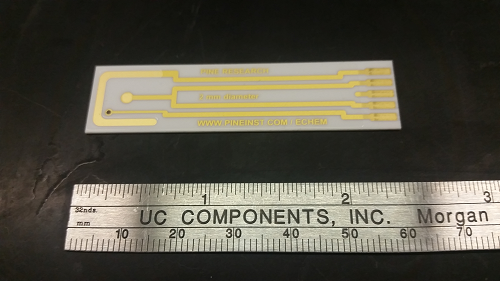
\includegraphics[width=3in]{./images/apparatus/electrode.png}
\caption{\label{fig-s8}Three-electrode system used for all experiments. A ruler was included for scale.}
\end{figure}

\subsection{Electrochemical Cell for LSV with Electrolyte Switching}
\label{sec-5-2}
Figure \ref{fig-s9} shows a top-view of the electrochemical cell used for the LSV electrolyte switching experiments. The patterned 3-electrode was connected to the white plug. The external Hg/HgO reference electrode is the clear plastic object with a black cap and white/blue tag.

\begin{figure}[h]
\centering
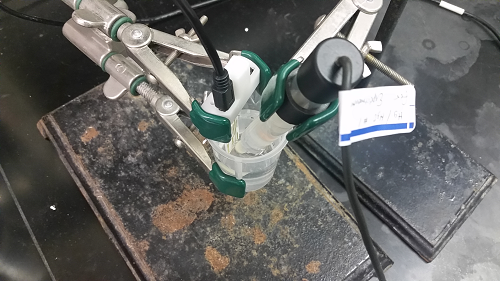
\includegraphics[width=3in]{./images/apparatus/ecell-bench-1.png}
\caption{\label{fig-s9}Electrochemical cell (top-view) used for LSV electrolyte switching experiments}
\end{figure}

Figure \ref{fig-s10} shows a side-view of the electrochemical cell shown above. This image provides a better view of the working and counter electrodes.
\begin{figure}[h]
\centering
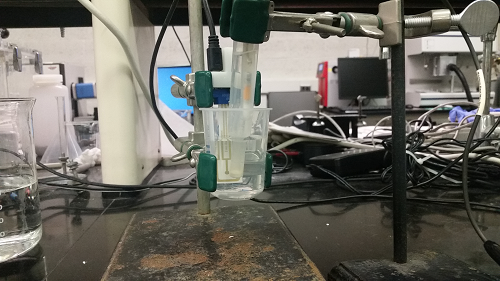
\includegraphics[width=3in]{./images/apparatus/ecell-bench-2.png}
\caption{\label{fig-s10}Electrochemical cell (side-view) used for LSV electrolyte switching experiments.}
\end{figure}
\subsection{Electrochemical Cell for LSV with Raman Spectroscopy}
\label{sec-5-3}
Figure \ref{fig-s11} shows the electrochemical cell mounted in the Raman spectroscopy system. This configuration was used to perform Raman spectroscopy during LSV. A laser beam was emitted from the black and blue objective above the electrode.
\begin{figure}[h]
\centering
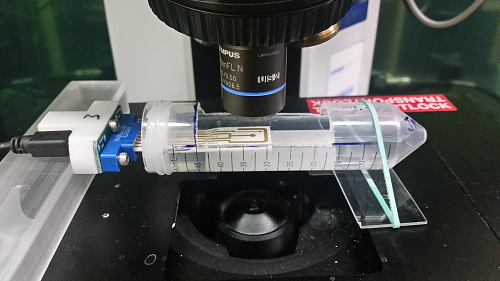
\includegraphics[width=3in]{./images/apparatus/ecell-raman.png}
\caption{\label{fig-s11}Electrochemical cell for performing LSV with Raman spectroscopy}
\end{figure}

\subsection{Ni(OH)$_{\text{2}}$ for Electrolyte Purification}
\label{sec-5-4}
Figure \ref{fig-s12} shows Ni(OH)$_{\text{2}}$ in a polypropylene vial for electrolyte purification \cite{trotochaud-2014-nickel-iron}. Stock electrolyte soaked in Ni(OH)$_{\text{2}}$ for at least 12 hours. The vial on the right shows electrolyte soaking in the adsorbent (i.e. Ni(OH)$_{\text{2}}$). The vial on the left shows purified electrolyte after centrifugation, but before it was collected into a separate polypropylene vial for storage.

\begin{figure}[h]
\centering
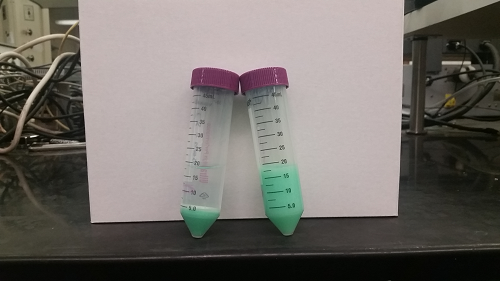
\includegraphics[width=3in]{./images/apparatus/ni-hydr-purif.png}
\caption{\label{fig-s12}Nickel hydroxide for electrolyte purification in plastic vials}
\end{figure}

\bibliographystyle{unsrt}
\bibliography{/Users/jkitchin/Desktop/cappa/kitchingroup-55/references}

\section{Appendix}
\label{sec-6}
\subsection{Code for Generating LSV Figures}
\label{sec-6-1}
\subsubsection{LSV with Electrolyte Switching in Purified LiOH and CsOH}
\label{sec-6-1-1}
\begin{minted}[frame=lines,fontsize=\scriptsize,linenos]{python}
# Generate I vs. V figure
# LSV: LiOH, CsOH (purified)
import numpy as np
import matplotlib.pyplot as plt
import xlrd
# Open I vs. V data file
ex1 = xlrd.open_workbook('./data/lsv-data/lsv-li-cs-pure-10-08-mod.xlsx')
ex2 = xlrd.open_workbook('./data/lsv-data/lsv-li-cs-pure-10-03-mod.xlsx')

# LiOH
Li1 = ex1.sheet_by_index(0)                           # read data from Excel sheet
Li2 = ex1.sheet_by_index(1)
Li3 = ex1.sheet_by_index(2)
Li4 = ex1.sheet_by_index(3)
Li5 = ex2.sheet_by_index(0)
Li6 = ex2.sheet_by_index(1)
Li7 = ex2.sheet_by_index(2)

x = np.array(Li1.col_values(0)) - 0.365               # convert potential to overpotential (V)

LiI1 = np.array(Li1.col_values(1)) * 1000/0.0314159   # convert current (A) to current density (mA/cm2)
LiI2 = np.array(Li2.col_values(1)) * 1000/0.0314159
LiI3 = np.array(Li3.col_values(1)) * 1000/0.0314159
LiI4 = np.array(Li4.col_values(1)) * 1000/0.0314159
LiI5 = np.array(Li5.col_values(1)) * 1000/0.0314159
LiI6 = np.array(Li6.col_values(1)) * 1000/0.0314159
LiI7 = np.array(Li7.col_values(1)) * 1000/0.0314159
LiI = np.array([LiI2, LiI3, LiI4, LiI5, LiI6, LiI7])

# CsOH
Cs1 = ex1.sheet_by_index(4)                           # read data from Excel sheet
Cs2 = ex1.sheet_by_index(5)
Cs3 = ex1.sheet_by_index(6)
Cs4 = ex1.sheet_by_index(7)
Cs5 = ex2.sheet_by_index(3)
Cs6 = ex2.sheet_by_index(4)
Cs7 = ex2.sheet_by_index(5)

CsI1 = np.array(Cs1.col_values(1)) * 1000/0.0314159   # convert current (A) to current density (mA/cm2)
CsI2 = np.array(Cs2.col_values(1)) * 1000/0.0314159
CsI3 = np.array(Cs3.col_values(1)) * 1000/0.0314159
CsI4 = np.array(Cs4.col_values(1)) * 1000/0.0314159
CsI5 = np.array(Cs5.col_values(1)) * 1000/0.0314159
CsI6 = np.array(Cs6.col_values(1)) * 1000/0.0314159
CsI7 = np.array(Cs7.col_values(1)) * 1000/0.0314159
CsI = np.array([CsI2, CsI3, CsI4, CsI5, CsI6, CsI7])

# Calculate average current density
avgLiI = (LiI2 + LiI3 + LiI4 + LiI5 + LiI6 + LiI7) / 6
avgCsI = (CsI2 + CsI3 + CsI4 + CsI5 + CsI6 + CsI7) / 6

# Calculate standard deviation of specified data points
nth = 80                                               # interval for calculating std. dev.
stdLi, stdCs = [], []
for n in LiI.T[::-nth]:
    stdLi.append(np.std(n))
stdLi = np.array(stdLi)

for n in CsI.T[::-nth]:
    stdCs.append(np.std(n))
stdCs = np.array(stdCs)

xx = x[::-nth]                                         # potentials where std. dev. calculated

# Generate and format figure
plt.figure(figsize=(3, 4))

plt.plot(x, avgCsI, 'r', label='CsOH')                 # voltage vs. avg. current density
plt.errorbar(xx, avgCsI[::-nth], yerr=stdCs, lw=0, elinewidth=1, color='r') # error bars
plt.plot(x, avgLiI, 'b', label='LiOH')
plt.errorbar(xx, avgLiI[::-nth], yerr=stdLi, lw=0, elinewidth=1, color='b')

plt.legend(loc='upper left', fontsize='11')            # legend
plt.xlabel('Overpotential (V)')                        # x-axis label
plt.ylabel('Current Density (mA/cm$^{2}$)')            # y-axis label
plt.axis([0.2, 0.6, -0.1, 3])                           # x,y axis values
plt.tight_layout()
plt.xticks([0.2, 0.3, 0.4, 0.5, 0.6], [0.2, 0.3, 0.4, 0.5, 0.6])

# Save image with various extentions
for ext in ['eps', 'pdf', 'png']:
    plt.savefig('./images/figures-supp-info/IvsV-Li-Cs-pure-10-08.{0}'.format(ext), dpi=300)

plt.show()
\end{minted}

\subsubsection{LSV with Electrolyte Switching in Fe-saturated LiOH and CsOH}
\label{sec-6-1-2}
\begin{minted}[frame=lines,fontsize=\scriptsize,linenos]{python}
#Generate I vs. V figure
#LiOH, CsOH - purified
import numpy as np
import matplotlib.pyplot as plt
import xlrd
# Open I vs. V data file
ex1 = xlrd.open_workbook('./data/lsv-data/lsv-li-cs-iron-11-21.xlsx')

# LiOH
Li1 = ex1.sheet_by_index(0)                           # read data from Excel sheet
Li2 = ex1.sheet_by_index(1)
Li3 = ex1.sheet_by_index(2)
Li4 = ex1.sheet_by_index(3)

x = np.array(Li1.col_values(0)) - 0.365               # potential to overpotential (V)

LiI1 = np.array(Li1.col_values(1)) * 1000/0.0314159   # current (A) to current density (mA/cm2)
LiI2 = np.array(Li2.col_values(1)) * 1000/0.0314159
LiI3 = np.array(Li3.col_values(1)) * 1000/0.0314159
LiI4 = np.array(Li4.col_values(1)) * 1000/0.0314159
LiI = np.array([LiI1, LiI2, LiI3, LiI4])

# CsOH
Cs1 = ex1.sheet_by_index(4)                           # read data from Excel sheet
Cs2 = ex1.sheet_by_index(5)
Cs3 = ex1.sheet_by_index(6)
Cs4 = ex1.sheet_by_index(7)

CsI1 = np.array(Cs1.col_values(1)) * 1000/0.0314159   # current (A) to current density (mA/cm2)
CsI2 = np.array(Cs2.col_values(1)) * 1000/0.0314159
CsI3 = np.array(Cs3.col_values(1)) * 1000/0.0314159
CsI4 = np.array(Cs4.col_values(1)) * 1000/0.0314159
CsI = np.array([CsI1, CsI2, CsI3, CsI4])

# Calculate average current density
avgLiI = (LiI1 + LiI2 + LiI3 + LiI4) / 4
avgCsI = (CsI1 + CsI2 + CsI3 + CsI4) / 4

# Calculate standard deviation of specified data points
nth = 60                                              # interval for calculating std. dev.
stdLi, stdCs = [], []
for n in LiI.T[::-nth]:
    stdLi.append(np.std(n))
stdLi = np.array(stdLi)

for n in CsI.T[::-nth]:
    stdCs.append(np.std(n))
stdCs = np.array(stdCs)

xx = x[::-nth]                                        # potentials where std. dev. calculated

# Generate and format figure
plt.figure(figsize=(3, 4))

plt.plot(x, avgCsI, 'r', label='CsOH')                #plot voltage vs. avg. current density
plt.errorbar(xx, avgCsI[::-nth], yerr=stdCs, lw=0, elinewidth=1, color='r') # error bars
plt.plot(x, avgLiI, 'b', label='LiOH')
plt.errorbar(xx, avgLiI[::-nth], yerr=stdLi, lw=0, elinewidth=1, color='b')

plt.legend(loc='upper left', fontsize='11')           # legend
plt.xlabel('Overpotential (V)')                       # x-axis label
plt.ylabel('Current Density (mA/cm$^{2}$)')           # y-axis label
plt.axis([0.0, 0.5, -1, 25])                          # x,y axis values
plt.tight_layout()
plt.xticks([0.0, 0.1, 0.2, 0.3, 0.4, 0.5], [0.0, 0.1, 0.2, 0.3, 0.4, 0.5])

# Save image with various extentions
for ext in ['eps', 'pdf', 'png']:
    plt.savefig('./images/figures-supp-info/IvsV-Li-Cs-iron-11-21.{0}'.format(ext), dpi=300)

plt.show()
\end{minted}

\subsubsection{LSV with Electrolyte Switching in Purified NaOH and KOH}
\label{sec-6-1-3}
\begin{minted}[frame=lines,fontsize=\scriptsize,linenos]{python}
# Generate I vs. V figure
# LSV: LiOH, CsOH (purified)
import numpy as np
import matplotlib.pyplot as plt
import xlrd
# Open I vs. V data file
ex1 = xlrd.open_workbook('./data/lsv-data/lsv-na-k-pure-01-16.xlsx')

# NaOH
Na1 = ex1.sheet_by_index(0)                          # read data from Excel sheet
Na2 = ex1.sheet_by_index(1)
Na3 = ex1.sheet_by_index(2)
Na4 = ex1.sheet_by_index(3)

x = np.array(Na1.col_values(0)) - 0.365              # potential to overpotential (V)

NaI1 = np.array(Na1.col_values(1)) * 1000/0.0314159  # current (A) to current density (mA/cm2)
NaI2 = np.array(Na2.col_values(1)) * 1000/0.0314159
NaI3 = np.array(Na3.col_values(1)) * 1000/0.0314159
NaI4 = np.array(Na4.col_values(1)) * 1000/0.0314159
NaI = np.array([NaI2, NaI3, NaI4])

# KOH
K1 = ex1.sheet_by_index(4)                           # read data from Excel sheet
K2 = ex1.sheet_by_index(5)
K3 = ex1.sheet_by_index(6)
K4 = ex1.sheet_by_index(7)

KI1 = np.array(K1.col_values(1)) * 1000/0.0314159    # current (A) to current density (mA/cm2)
KI2 = np.array(K2.col_values(1)) * 1000/0.0314159
KI3 = np.array(K3.col_values(1)) * 1000/0.0314159
KI4 = np.array(K4.col_values(1)) * 1000/0.0314159
KI = np.array([KI2, KI3, KI4])

# Calculate average current density
avgNaI = (NaI2 + NaI3 + NaI4) / 3
avgKI = (KI2 + KI3 + KI4) / 3

# Calculate standard deviation of specified data points
nth = 70                                             # interval for calculating std. dev.
stdNa, stdK = [], []
for n in NaI.T[::-nth]:
    stdNa.append(np.std(n))
stdNa = np.array(stdNa)

for n in KI.T[::-nth]:
    stdK.append(np.std(n))
stdK = np.array(stdK)
xx = x[::-nth]                                      # potentials where std. dev. calculated

# Generate and format figure
plt.figure(figsize=(3, 4))

plt.plot(x, avgKI, 'k', label='KOH')                #plot voltage vs. avg. current density
plt.errorbar(xx, avgKI[::-nth], yerr=stdK, lw=0, elinewidth=1, color='k') # error bars
plt.plot(x, avgNaI, 'g', label='NaOH')
plt.errorbar(xx, avgNaI[::-nth], yerr=stdNa, lw=0, elinewidth=1, color='g')

plt.legend(loc='upper left', fontsize='11')         # legend
plt.xlabel('Overpotential (V)')                     # x-axis label
plt.ylabel('Current Density (mA/cm$^{2}$)')         # y-axis label
plt.axis([0.2, 0.6, -0.1, 2])                       # x,y axis values
plt.tight_layout()
plt.xticks([0.2, 0.3, 0.4, 0.5, 0.6], [0.2, 0.3, 0.4, 0.5, 0.6])

# Save image with various extentions
for ext in ['eps', 'pdf', 'png']:
    plt.savefig('./images/figures-supp-info/IvsV-Na-K-pure-01-16-15.{0}'.format(ext), dpi=300)

plt.show()
\end{minted}

\subsubsection{LSV with Electrolyte Switching in Fe-saturated NaOH and KOH}
\label{sec-6-1-4}
\begin{minted}[frame=lines,fontsize=\scriptsize,linenos]{python}
# Generate I vs. V figure
# LSV: NaOH, KOH (Fe-saturated)
import numpy as np
import matplotlib.pyplot as plt
import xlrd
# Open I vs. V data file
ex1 = xlrd.open_workbook('./data/lsv-data/lsv-na-k-iron-01-19.xlsx')

# NaOH
Na1 = ex1.sheet_by_index(0)                          # read data from Excel sheet
Na2 = ex1.sheet_by_index(1)
Na3 = ex1.sheet_by_index(2)
Na4 = ex1.sheet_by_index(3)

x = np.array(Na1.col_values(0)) - 0.365              # potential to overpotential (V)

NaI1 = np.array(Na1.col_values(1)) * 1000/0.0314159  # current (A) to current density (mA/cm2)
NaI2 = np.array(Na2.col_values(1)) * 1000/0.0314159
NaI3 = np.array(Na3.col_values(1)) * 1000/0.0314159
NaI4 = np.array(Na4.col_values(1)) * 1000/0.0314159
NaI = np.array([NaI2, NaI3, NaI4])

# KOH
K1 = ex1.sheet_by_index(4)                           # read data from Excel sheet
K2 = ex1.sheet_by_index(5)
K3 = ex1.sheet_by_index(6)
K4 = ex1.sheet_by_index(7)

KI1 = np.array(K1.col_values(1)) * 1000/0.0314159    # current (A) to current density (mA/cm2)
KI2 = np.array(K2.col_values(1)) * 1000/0.0314159
KI3 = np.array(K3.col_values(1)) * 1000/0.0314159
KI4 = np.array(K4.col_values(1)) * 1000/0.0314159
KI = np.array([KI2, KI3, KI4])

# Calculate average current density
avgNaI = (NaI2 + NaI3 + NaI4) / 3
avgKI = (KI2 + KI3 + KI4) / 3

# Calculate standard deviation of specified data points
nth = 70                                            # interval for calculating std. dev.
stdNa, stdK = [], []
for n in NaI.T[::-nth]:
    stdNa.append(np.std(n))
stdNa = np.array(stdNa)

for n in KI.T[::-nth]:
    stdK.append(np.std(n))
stdK = np.array(stdK)
xx = x[::-nth]                                      # potentials where std. dev. calculated

# Generate and format figure
plt.figure(figsize=(3, 4))

plt.plot(x, avgKI, 'k', label='KOH')               # voltage vs. avg. current density
plt.errorbar(xx, avgKI[::-nth], yerr=stdK, lw=0, elinewidth=1, color='k') # error bars
plt.plot(x, avgNaI, 'g', label='NaOH')
plt.errorbar(xx, avgNaI[::-nth], yerr=stdNa, lw=0, elinewidth=1, color='g')

plt.legend(loc='upper left', fontsize='11')        # legend
plt.xlabel('Overpotential (V)')                    # x-axis label
plt.ylabel('Current Density (mA/cm$^{2}$)')        # y-axis label
plt.axis([0.0, 0.5, -1, 30])                       # x,y axis values
plt.tight_layout()
plt.xticks([0.0, 0.1, 0.2, 0.3, 0.4, 0.5], [0.0, 0.1, 0.2, 0.3, 0.4, 0.5])

# Save image with various extentions
for ext in ['eps', 'pdf', 'png']:
    plt.savefig('./images/figures-supp-info/IvsV-Na-K-iron-01-19.{0}'.format(ext), dpi=300)

plt.show()
\end{minted}

\subsubsection{LSV with Electrolyte Switching in Purified LiOH, NaOH, KOH, and CsOH}
\label{sec-6-1-5}
\begin{minted}[frame=lines,fontsize=\scriptsize,linenos]{python}
# Generate I vs. V figure
# LSV; LiOH, CsOH (purified)
import numpy as np
import matplotlib.pyplot as plt
import xlrd
# Open I vs. V data file
ex1 = xlrd.open_workbook('./data/lsv-data/lsv-li-cs-pure-10-08-mod.xlsx')
ex2 = xlrd.open_workbook('./data/lsv-data/lsv-li-cs-pure-10-03-mod.xlsx')
ex3 = xlrd.open_workbook('./data/lsv-data/lsv-na-k-pure-01-16.xlsx')

# LiOH
Li1 = ex1.sheet_by_index(0)                          # read data from Excel sheet
Li2 = ex1.sheet_by_index(1)
Li3 = ex1.sheet_by_index(2)
Li4 = ex1.sheet_by_index(3)
Li5 = ex2.sheet_by_index(0)
Li6 = ex2.sheet_by_index(1)
Li7 = ex2.sheet_by_index(2)

x = np.array(Li1.col_values(0)) - 0.365              # potential to overpotential (V)

LiI1 = np.array(Li1.col_values(1)) * 1000/0.0314159  # current (A) to current density (mA/cm2)
LiI2 = np.array(Li2.col_values(1)) * 1000/0.0314159
LiI3 = np.array(Li3.col_values(1)) * 1000/0.0314159
LiI4 = np.array(Li4.col_values(1)) * 1000/0.0314159
LiI5 = np.array(Li5.col_values(1)) * 1000/0.0314159
LiI6 = np.array(Li6.col_values(1)) * 1000/0.0314159
LiI7 = np.array(Li7.col_values(1)) * 1000/0.0314159
LiI = np.array([LiI2, LiI3, LiI4, LiI5, LiI6, LiI7])

# CsOH
Cs1 = ex1.sheet_by_index(4)                           # read data from Excel sheet
Cs2 = ex1.sheet_by_index(5)
Cs3 = ex1.sheet_by_index(6)
Cs4 = ex1.sheet_by_index(7)
Cs5 = ex2.sheet_by_index(3)
Cs6 = ex2.sheet_by_index(4)
Cs7 = ex2.sheet_by_index(5)

CsI1 = np.array(Cs1.col_values(1)) * 1000/0.0314159   # current (A) to current density (mA/cm2)
CsI2 = np.array(Cs2.col_values(1)) * 1000/0.0314159
CsI3 = np.array(Cs3.col_values(1)) * 1000/0.0314159
CsI4 = np.array(Cs4.col_values(1)) * 1000/0.0314159
CsI5 = np.array(Cs5.col_values(1)) * 1000/0.0314159
CsI6 = np.array(Cs6.col_values(1)) * 1000/0.0314159
CsI7 = np.array(Cs7.col_values(1)) * 1000/0.0314159
CsI = np.array([CsI2, CsI3, CsI4, CsI5, CsI6, CsI7])

# NaOH
Na1 = ex3.sheet_by_index(0)                           # read data from Excel sheet
Na2 = ex3.sheet_by_index(1)
Na3 = ex3.sheet_by_index(2)
Na4 = ex3.sheet_by_index(3)

x = np.array(Na1.col_values(0)) - 0.365               # potential to overpotential (V)

NaI1 = np.array(Na1.col_values(1)) * 1000/0.0314159   # current (A) to current density (mA/cm2)
NaI2 = np.array(Na2.col_values(1)) * 1000/0.0314159
NaI3 = np.array(Na3.col_values(1)) * 1000/0.0314159
NaI4 = np.array(Na4.col_values(1)) * 1000/0.0314159
NaI = np.array([NaI2, NaI3, NaI4])

# KOH
K1 = ex3.sheet_by_index(4)                            # read data from Excel sheet
K2 = ex3.sheet_by_index(5)
K3 = ex3.sheet_by_index(6)
K4 = ex3.sheet_by_index(7)

KI1 = np.array(K1.col_values(1)) * 1000/0.0314159     # current (A) to current density (mA/cm2)
KI2 = np.array(K2.col_values(1)) * 1000/0.0314159
KI3 = np.array(K3.col_values(1)) * 1000/0.0314159
KI4 = np.array(K4.col_values(1)) * 1000/0.0314159
KI = np.array([KI2, KI3, KI4])

# Calculate average current density
avgLiI = (LiI2 + LiI3 + LiI4 + LiI5 + LiI6 + LiI7) / 6
avgCsI = (CsI2 + CsI3 + CsI4 + CsI5 + CsI6 + CsI7) / 6
avgNaI = (NaI2 + NaI3 + NaI4) / 3
avgKI = (KI2 + KI3 + KI4) / 3

# Calculate standard deviation of specified data points
nth = 80                                               # interval for calculating std. dev.
stdLi, stdCs, stdNa, stdK = [], [], [], []
for n in LiI.T[::-nth]:
    stdLi.append(np.std(n))
stdLi = np.array(stdLi)

for n in CsI.T[::-nth]:
    stdCs.append(np.std(n))
stdCs = np.array(stdCs)

for n in NaI.T[::-nth]:
    stdNa.append(np.std(n))
stdNa = np.array(stdNa)

for n in KI.T[::-nth]:
    stdK.append(np.std(n))
stdK = np.array(stdK)

xx = x[::-nth]

# Generate and format figure
plt.figure(figsize=(3, 4))

plt.plot(x, avgCsI, 'r', label='CsOH')
plt.errorbar(xx, avgCsI[::-nth], yerr=stdCs, lw=0, elinewidth=1, color='r')

plt.plot(x, avgKI, 'k', label='KOH')            #plot voltage vs. avg. current density
plt.errorbar(xx, avgKI[::-nth], yerr=stdK, lw=0, elinewidth=1, color='k') # error bars

plt.plot(x, avgNaI, 'g', label='NaOH')
plt.errorbar(xx, avgNaI[::-nth], yerr=stdNa, lw=0, elinewidth=1, color='g')

plt.plot(x, avgLiI, 'b', label='LiOH')
plt.errorbar(xx, avgLiI[::-nth], yerr=stdLi, lw=0, elinewidth=1, color='b')

plt.legend(loc='upper left', fontsize='11')       # legend
plt.xlabel('Overpotential (V)')                   # x-axis label
plt.ylabel('Current Density (mA/cm$^{2}$)')       # y-axis label
plt.axis([0.2, 0.6, -0.1, 3])                       # x,y axis values
plt.tight_layout()
plt.xticks([0.2, 0.3, 0.4, 0.5, 0.6], [0.2, 0.3, 0.4, 0.5, 0.6])

# Save image with various extentions
for ext in ['eps', 'pdf', 'png']:
    plt.savefig('./images/figures-main/IvsV-Na-K-Li-Cs-pure.{0}'.format(ext), dpi=300)

plt.show()
\end{minted}

\subsubsection{LSV with Electrolyte Switching in Fe-saturated LiOH, NaOH, KOH, and CsOH}
\label{sec-6-1-6}
\begin{minted}[frame=lines,fontsize=\scriptsize,linenos]{python}
# Generate I vs. V figure
# LSV: LiOH, NaOH, KOH, CsOH (Fe-saturated)
import numpy as np
import matplotlib.pyplot as plt
import xlrd
# Open I vs. V data file
ex1 = xlrd.open_workbook('./data/lsv-data/lsv-li-cs-iron-11-21.xlsx')
ex2 = xlrd.open_workbook('./data/lsv-data/lsv-na-k-iron-01-19.xlsx')

# LiOH
Li1 = ex1.sheet_by_index(0)                          # read data from Excel sheet
Li2 = ex1.sheet_by_index(1)
Li3 = ex1.sheet_by_index(2)
Li4 = ex1.sheet_by_index(3)

x = np.array(Li1.col_values(0)) - 0.365               # potential to overpotential (V)

LiI1 = np.array(Li1.col_values(1)) * 1000/0.0314159   # current (A) to current density (mA/cm2)
LiI2 = np.array(Li2.col_values(1)) * 1000/0.0314159
LiI3 = np.array(Li3.col_values(1)) * 1000/0.0314159
LiI4 = np.array(Li4.col_values(1)) * 1000/0.0314159
LiI = np.array([LiI1, LiI2, LiI3, LiI4])

# CsOH
Cs1 = ex1.sheet_by_index(4)                           # read data from Excel sheet
Cs2 = ex1.sheet_by_index(5)
Cs3 = ex1.sheet_by_index(6)
Cs4 = ex1.sheet_by_index(7)

CsI1 = np.array(Cs1.col_values(1)) * 1000/0.0314159   # current (A) to current density (mA/cm2)
CsI2 = np.array(Cs2.col_values(1)) * 1000/0.0314159
CsI3 = np.array(Cs3.col_values(1)) * 1000/0.0314159
CsI4 = np.array(Cs4.col_values(1)) * 1000/0.0314159
CsI = np.array([CsI1, CsI2, CsI3, CsI4])

# NaOH
Na1 = ex2.sheet_by_index(0)                           # read data from Excel sheet
Na2 = ex2.sheet_by_index(1)
Na3 = ex2.sheet_by_index(2)
Na4 = ex2.sheet_by_index(3)

x = np.array(Na1.col_values(0)) - 0.365               # potential to overpotential (V)

NaI1 = np.array(Na1.col_values(1)) * 1000/0.0314159   # current (A) to current density (mA/cm2)
NaI2 = np.array(Na2.col_values(1)) * 1000/0.0314159
NaI3 = np.array(Na3.col_values(1)) * 1000/0.0314159
NaI4 = np.array(Na4.col_values(1)) * 1000/0.0314159
NaI = np.array([NaI2, NaI3, NaI4])

# KOH
K1 = ex2.sheet_by_index(4)                            # read data from Excel sheet
K2 = ex2.sheet_by_index(5)
K3 = ex2.sheet_by_index(6)
K4 = ex2.sheet_by_index(7)

KI1 = np.array(K1.col_values(1)) * 1000/0.0314159     # current (A) to current density (mA/cm2)
KI2 = np.array(K2.col_values(1)) * 1000/0.0314159
KI3 = np.array(K3.col_values(1)) * 1000/0.0314159
KI4 = np.array(K4.col_values(1)) * 1000/0.0314159
KI = np.array([KI2, KI3, KI4])

# Calculate average current density
avgLiI = (LiI1 + LiI2 + LiI3 + LiI4) / 4
avgCsI = (CsI1 + CsI2 + CsI3 + CsI4) / 4
avgNaI = (NaI2 + NaI3 + NaI4) / 3
avgKI = (KI2 + KI3 + KI4) / 3

# Calculate standard deviation of specified data points
nth = 80                                               # interval for calculating std. dev.
stdLi, stdCs, stdNa, stdK = [], [], [], []

for n in LiI.T[::-nth]:
    stdLi.append(np.std(n))
stdLi = np.array(stdLi)

for n in CsI.T[::-nth]:
    stdCs.append(np.std(n))
stdCs = np.array(stdCs)

for n in NaI.T[::-nth]:
    stdNa.append(np.std(n))
stdNa = np.array(stdNa)

for n in KI.T[::-nth]:
    stdK.append(np.std(n))
stdK = np.array(stdK)

xx = x[::-nth]

# Generate and format figure
plt.figure(figsize=(3, 4))

plt.plot(x, avgKI, 'k', label='KOH')                  #plot voltage vs. avg. current density
plt.errorbar(xx, avgKI[::-nth], yerr=stdK, lw=0, elinewidth=1, color='k') # error bars

plt.plot(x, avgNaI, 'g', label='NaOH')
plt.errorbar(xx, avgNaI[::-nth], yerr=stdNa, lw=0, elinewidth=1, color='g')

plt.plot(x, avgCsI, 'r', label='CsOH')
plt.errorbar(xx, avgCsI[::-nth], yerr=stdCs, lw=0, elinewidth=1, color='r')

plt.plot(x, avgLiI, 'b', label='LiOH')
plt.errorbar(xx, avgLiI[::-nth], yerr=stdLi, lw=0, elinewidth=1, color='b')

plt.legend(loc='upper left', fontsize='11')          # legend
plt.xlabel('Overpotential (V)')                      # x-axis label
plt.ylabel('Current Density (mA/cm$^{2}$)')          # y-axis label
plt.axis([0.0, 0.6, -1, 30])                         # x,y axis values
plt.tight_layout()
plt.xticks([0.0, 0.1, 0.2, 0.3, 0.4, 0.5, 0.6], [0.0, 0.1, 0.2, 0.3, 0.4, 0.5, 0.6])

# Save image with various extentions
for ext in ['eps', 'pdf', 'png']:
    plt.savefig('./images/figures-main/IvsV-Na-K-Li-Cs-iron.{0}'.format(ext), dpi=300)

plt.show()
\end{minted}

\subsubsection{LSV during Raman Spectroscopy in Purified LiOH and CsOH}
\label{sec-6-1-7}
\begin{minted}[frame=lines,fontsize=\scriptsize,linenos]{python}
# Generate I vs. V figure
# LSV during Raman spectroscopy: LiOH, CsOH (purified)
import numpy as np
import matplotlib.pyplot as plt
import xlrd
# Open I vs. V data file
ex1 = xlrd.open_workbook('./data/lsv-data/lsv-raman-li-cs-pure-10-31.xlsx')

# LiOH
Li1 = ex1.sheet_by_index(0)                            # read data from Excel sheet
Li2 = ex1.sheet_by_index(1)
Li3 = ex1.sheet_by_index(2)
Li4 = ex1.sheet_by_index(3)

x = np.array(Li1.col_values(0)) - 0.365                # potential to overpotential (V)

LiI1 = np.array(Li1.col_values(1)) * 1000/0.0314159    # current (A) to current density (mA/cm2)
LiI2 = np.array(Li2.col_values(1)) * 1000/0.0314159
LiI3 = np.array(Li3.col_values(1)) * 1000/0.0314159
LiI4 = np.array(Li4.col_values(1)) * 1000/0.0314159
LiI = np.array([LiI2, LiI3, LiI4])

# CsOH
Cs1 = ex1.sheet_by_index(4)                            # read data from Excel sheet
Cs2 = ex1.sheet_by_index(5)
Cs3 = ex1.sheet_by_index(6)
Cs4 = ex1.sheet_by_index(7)

#CsV1 = np.array(Cs1.col_values(0)) - 0.365            # potential to overpotential (V)
CsI1 = np.array(Cs1.col_values(1)) * 1000/0.0314159    # current (A) to current density (mA/cm2)
CsI2 = np.array(Cs2.col_values(1)) * 1000/0.0314159
CsI3 = np.array(Cs3.col_values(1)) * 1000/0.0314159
CsI4 = np.array(Cs4.col_values(1)) * 1000/0.0314159
CsI = np.array([CsI2, CsI3, CsI4])

# Calculate average current density
avgLiI = (LiI2 + LiI3 + LiI4) / 3
avgCsI = (CsI2 + CsI3 + CsI4) / 3

# Calculate standard deviation of specified data points
nth = 80                                               # interval for calculating std. dev.
stdLi, stdCs = [], []
for n in LiI.T[::-nth]:
    stdLi.append(np.std(n))
stdLi = np.array(stdLi)

for n in CsI.T[::-nth]:
    stdCs.append(np.std(n))
stdCs = np.array(stdCs)

xx = x[::-nth]                                         # potentials where std. dev. calculated

# Generate and format figure
plt.figure(figsize=(3, 4))

plt.plot(x, avgCsI, 'r', label='CsOH')                 # plot voltage vs. avg. current density
plt.errorbar(xx, avgCsI[::-nth], yerr=stdCs, lw=0, elinewidth=1, color='r') # error bars
plt.plot(x, avgLiI, 'b', label='LiOH')
plt.errorbar(xx, avgLiI[::-nth], yerr=stdLi, lw=0, elinewidth=1, color='b')

plt.legend(loc='upper left', fontsize='11')            # legend
plt.xlabel('Overpotential (V)')                        # x-axis label
plt.ylabel('Current Density (mA/cm$^{2}$)')            # y-axis label
plt.axis([0.2, 0.6, -0.1, 8])                          # x,y axis values
plt.tight_layout()
plt.xticks([0.2, 0.3, 0.4, 0.5, 0.6], [0.2, 0.3, 0.4, 0.5, 0.6])

# Save image with various extentions
for ext in ['eps', 'pdf', 'png']:
    plt.savefig('./images/figures-supp-info/IvsV-Raman-Li-Cs-pure-10-31.{0}'.format(ext), dpi=300)

plt.show()
\end{minted}

\subsubsection{LSV during Raman Spectroscopy in Fe-saturated LiOH and CsOH}
\label{sec-6-1-8}
\begin{minted}[frame=lines,fontsize=\scriptsize,linenos]{python}
# Generate I vs. V figure
# LSV during Raman spectroscopy: LiOH, CsOH (Fe-saturated)
import numpy as np
import matplotlib.pyplot as plt
import xlrd
# Open I vs. V data file
ex1 = xlrd.open_workbook('./data/lsv-data/lsv-raman-li-cs-iron-11-19.xlsx')

# LiOH
Li1 = ex1.sheet_by_index(0)                           # read data from Excel sheet
Li2 = ex1.sheet_by_index(1)
Li3 = ex1.sheet_by_index(2)
Li4 = ex1.sheet_by_index(3)

x = np.array(Li1.col_values(0)) - 0.365               # potential to overpotential (V)

LiI1 = np.array(Li1.col_values(1)) * 1000/0.0314159   # current (A) to current density (mA/cm2)
LiI2 = np.array(Li2.col_values(1)) * 1000/0.0314159
LiI3 = np.array(Li3.col_values(1)) * 1000/0.0314159
LiI4 = np.array(Li4.col_values(1)) * 1000/0.0314159
LiI = np.array([LiI1, LiI3, LiI4])

# CsOH
Cs1 = ex1.sheet_by_index(4)                           # read data from Excel sheet
Cs2 = ex1.sheet_by_index(5)
Cs3 = ex1.sheet_by_index(6)
Cs4 = ex1.sheet_by_index(7)

CsI1 = np.array(Cs1.col_values(1)) * 1000/0.0314159   # current (A) to current density (mA/cm2)
CsI2 = np.array(Cs2.col_values(1)) * 1000/0.0314159
CsI3 = np.array(Cs3.col_values(1)) * 1000/0.0314159
CsI4 = np.array(Cs4.col_values(1)) * 1000/0.0314159
CsI = np.array([CsI1, CsI2, CsI3, CsI4])

# Calculate average current density
avgLiI = (LiI1 + LiI3 + LiI4) / 3
avgCsI = (LiI1 + CsI2 + CsI3 + CsI4) / 4

# Calculate standard deviation of specified data points
nth = 80                                               # interval for calculating std. dev.
stdLi, stdCs = [], []
for n in LiI.T[::-nth]:
    stdLi.append(np.std(n))
stdLi = np.array(stdLi)

for n in CsI.T[::-nth]:
    stdCs.append(np.std(n))
stdCs = np.array(stdCs)

xx = x[::-nth]

# Generate and format figure
plt.figure(figsize=(3, 4))

plt.plot(x, avgCsI, 'r', label='CsOH')                 # plot voltage vs. avg. current density
plt.errorbar(xx, avgCsI[::-nth], yerr=stdCs, lw=0, elinewidth=1, color='r') # error bars
plt.plot(x, avgLiI, 'b', label='LiOH')
plt.errorbar(xx, avgLiI[::-nth], yerr=stdLi, lw=0, elinewidth=1, color='b')

plt.legend(loc='upper left', fontsize='11')            # legend
plt.xlabel('Overpotential (V)')                        # x-axis label
plt.ylabel('Current Density (mA/cm$^{2}$)')            # y-axis label
plt.axis([0.0, 0.6, -1, 16])                           # x,y axis values
plt.tight_layout()
plt.xticks([0.0, 0.2, 0.4, 0.6], [0.0, 0.2, 0.4, 0.6])

# Save image with various extentions
for ext in ['eps', 'pdf', 'png']:
    plt.savefig('./images/figures-supp-info/IvsV-Raman-Li-Cs-iron-11-19.{0}'.format(ext), dpi=300)

plt.show()
\end{minted}

\subsection{Code for Raman Peak Fitting}
\label{sec-6-2}
Below is a Python function for fitting Gaussian distributions to Raman spectra of NiOOH thin films. This function was called in other Python code blocks within this Supporting Information file. See section \ref{sec-4}.

\begin{minted}[frame=lines,fontsize=\scriptsize,linenos]{python}
import numpy as np
import matplotlib.pyplot as plt
from scipy.special import erf
from scipy.optimize import curve_fit
import os

def dgaus2p(filename,
            cntr=(470.0, 560.0),
            amp1=(20.0, 20.0),
            amp2=(20.0, 20.0),
            std1=(10.0, 5.0),
            std2=(10.0, 5.0),
            datarange=None,
            output=False,
            step=4):

    """Fitting Raman spectra data using the two Gaussian functions

    This function fits two double Gaussian fits for Raman peaks
    with overlapping tails.

    Parameters
    ----------
    filename : str
        The name of the file containing the data to be analyzed. Data is
        read in using the numpy.loadtxt function. Data should be separated
        into two rows, the first being the wavenumber, the second being
        signal intensity.

    cntr : list, optional
        Initial starting point for the center of each peak in wavenumbers.
        A float in the list for each peak.

    amp1 : list, optional
        Initial starting point for the amplitude of the frist Gaussian.
        A float in the list for each peak.

    amp2 : list, optional
        Initial starting point for the amplitude of the second Gaussian.
        A float in the list for each peak.

    std1 : list, optional
        Initial starting point for the standard deviation of the frist
        Gaussian. A float in the list for each peak.

    std2 : list, optional
        Initial starting point for the standard deviation of the second
        Gaussian. A float in the list for each peak.

    datarange : list, optional
        This is a list of two floats specifying the range of wavenumbers
        you want to analyze from the data file. Takes the entire range of
        data by default.

    output : bool , optional
        Whether or not the function returns an output .fit file.

    step : 1, 2, 3, or 4 : optional
        Specifies which step of the fitting process the user is working on:
        step = 1: Fittings the baseline (figure produced)
        step = 2: Choosing initial guess for peaks (figure produced)
        step = 3: Evaluate the fit (figure produced)
        step = 4: View and save the final figure (no figure)


    Returns
    -------
    results : array
        An array of: [center peak 1, center peak 2,
                      height peak 1, height peak 2,
                      area peak 1, area peak 2,
                      baseline slope, baseline intercept]

    fiterror : array
        An array of the fitting errors for: [center peak 1, center peak 2,
                                             height peak 1, height peak 2]

    popt : array
        An array of the optimized fitting parameters as output from the
        scipy.optimize.curve_fit function:
        Peak # :  1        2
                 [cntr[0], cntr[1],   # Peak center
                  amp1[0], amp1[1],   # Amplitude of Gaussian 1
                  amp2[0], amp2[1],   # Amplitude of Gaussian 2
                  std1[0], std1[1],   # Standard deviation of Gaussian 1
                  std2[0], std2[1])   # Standard deviation of Gaussian 2

    parguess : array
        An array of the initial fitting parameters:
        Peak # :  1        2
                 [cntr[0], cntr[1],   # Peak center
                  amp1[0], amp1[1],   # Amplitude of Gaussian 1
                  amp2[0], amp2[1],   # Amplitude of Gaussian 2
                  std1[0], std1[1],   # Standard deviation of Gaussian 1
                  std2[0], std2[1])   # Standard deviation of Gaussian 2

    See Also
    --------
    scipy.special.erf
    scipy.optimize.curve_fit
    """

    # This unpacks the data from the text file.
    S, I = np.loadtxt(filename, usecols=(0, 1), unpack=True)

    if datarange == None:
        datarange = [min(S), max(S)]

    # Define the low and high regions for baseline sampling
    dx = 80.
    low = datarange[0] + dx
    high = datarange[1] - dx

    # Seperate the data points to be used for fitting the baseline
    xbl = np.append(S[(S < low)], S[(S > high)])
    ybl = np.append(I[(S < low)], I[(S > high)])

    # Fits a line to the base line points
    blpars = np.polyfit(xbl, ybl, 1)
    blfit = np.poly1d(blpars)


    if step != 1 and step != 2 and step != 3 and step != 4:
        print 'Set step = 1, 2, 3, or 4 to continue'

    # Step 1: Choose low and high values for a satisfactory baseline
    if step == 1:
        plt.figure()
        plt.plot(S, I, label='data')
        plt.plot(S, blfit(S), 'r-', lw=2, label='base line')
        plt.xlabel('Raman shift (cm$^{-1}$)')
        plt.ylabel('Intensity (counts)')
        plt.legend(loc='best')
        plt.show()
        print 'When you are satisfied with the fit of the base line, set step = 2'
        exit()

    # Subtracts the baseline from the intensities
    I -= blfit(S)

    # Gaussians will only be fit the the data not used for the baseline
    nS = S[(S > low) & (S < high)]
    nI = I[(S > low) & (S < high)]

    # These are functions which define the types of fit which you could implement
    # Currently, the code only utilizes Gaussians
    # ----------------------------------------------------------------------
    def gaussian(x, pars):
        A = pars[0]    # amplitude
        mu = pars[1]   # means
        sig = pars[2]  # std dev
        return A * np.exp((-(x - mu)**2.) / ((2*sig)**2.))

    def sum_gaussian(x, *p):
        g1 = gaussian(x, [p[2], p[0], p[6]])
        g2 = gaussian(x, [p[3], p[0], p[7]])
        g3 = gaussian(x, [p[4], p[1], p[8]])
        g4 = gaussian(x, [p[5], p[1], p[9]])
        return g1 + g2 + g3 + g4
    # ----------------------------------------------------------------------

    # These are initial guesses of the tuning parameters for the Gaussian fits.
    # Peak # :  1        2
    parguess = (cntr[0], cntr[1],   # Peak center
                amp1[0], amp1[1],   # Amplitude of Gaussian 1
                amp2[0], amp2[1],   # Amplitude of Gaussian 2
                std1[0], std1[1],   # Standard deviation of Gaussian 1
                std2[0], std2[1])   # Standard deviation of Gaussian 2

    # Step 2: Fitting the curves to the data
    if step == 2:
        plt.figure()
        plt.plot(nS, nI, 'b-', label='Data')
        plt.plot(S, sum_gaussian(S, *parguess), 'g--', lw=3, label='Initial guess')
        plt.xlim(datarange[0], datarange[1])
        plt.ylim(0, max(nI) + 2)
        plt.xlabel('Raman shift (cm$^{-1}$)')
        plt.ylabel('Intensity (counts)')
        plt.legend(loc='best')
        plt.show()
        print 'Once the initial guess looks reasonable, set step = 3'
        exit()

    # This is a multivaraible curve fitting program which attempts to optimize the fitting parameters
    popt, pcov = curve_fit(sum_gaussian, S, I, parguess)

    peak1 = gaussian(S, [popt[2], popt[0], popt[6]]) + gaussian(S, [popt[3], popt[0], popt[7]])
    peak2 = gaussian(S, [popt[4], popt[1], popt[8]]) + gaussian(S, [popt[5], popt[1], popt[9]])

    # Step 3: Evaluate the fit
    if step == 3:
        plt.figure()
        plt.plot(nS, nI, 'b-', label='Data')
        plt.plot(S, sum_gaussian(S, *popt), 'r-', lw=3, label='Final Fit')
        plt.plot(S, peak1, 'm-', lw=3, label='Fit for peak 1')
        plt.plot(S, gaussian(S, [popt[4], popt[1], popt[8]]) + gaussian(S, [popt[5], popt[1], popt[9]]),
                 'c-', lw=3, label='Fit for peak 2')
        plt.xlim(low, high)
        plt.ylim(0, max(nI) + 2)
        plt.xlabel('Raman shift (cm$^{-1}$)')
        plt.ylabel('Intensity (counts)')
        plt.legend(loc='best')
        plt.show()
        print 'When you are satisfied with the peak fit, set step = 3'
        print 'else, return to step 2 and choose new fitting parameters'
        exit()

    # Step 4: A summary of the resulting fit
    if step == 4:
        ypeak1 = popt[2] + popt[3] + blfit(popt[0])
        ypeak2 = popt[4] + popt[5] + blfit(popt[1])

        area1 = -np.trapz(S, peak1)
        area2 = -np.trapz(S, peak2)

        savefile = filename.rstrip('txt')

        perr = np.sqrt(np.diag(pcov))

        pk1err = np.sqrt(perr[2]**2. + perr[3]**2 + 2 * pcov[2][3])
        pk2err = np.sqrt(perr[4]**2. + perr[5]**2 + 2 * pcov[4][5])

        results = np.array([popt[0], popt[1],
                            ypeak1, ypeak2,
                            area1, area2,
                            blpars[0], blpars[1]])

        fiterror = np.array([perr[0], perr[1],
                             pk1err, pk2err])

        if output:
            savefile = savefile + 'fit'

            f = 'Initial guess parameters:\n'
            f += '=========================\n'
            f += '                      Peak 1, Peak 2\n'
            f += 'Peak center =         {0:1.1f}, {1:1.2f}\n'.format(cntr[0], cntr[1])
            f += 'Amplitude fit 1 =     {0:1.1f}, {1:1.2f}\n'.format(amp1[0], amp1[1])
            f += 'Amplitude fit 2 =     {0:1.1f}, {1:1.2f}\n'.format(amp2[0], amp2[1])
            f += 'Standard dev. fit 1 = {0:1.1f}, {1:1.1f}\n'.format(std1[0], std1[1])
            f += 'Standard dev. fit 2 = {0:1.1f}, {1:1.1f}\n'.format(std2[0], std2[1])

            f += '\nBaseline parameters:\n'
            f += '===================\n'
            f += 'Slope =               {0:1.2f}\n'.format(blpars[0])
            f += 'Intercept =           {0:1.2f}\n'.format(blpars[1])

            f += '\nFitted parameters:\n'
            f += '==================\n'
            f += '                      Peak 1, Peak 2\n'
            f += 'Peak center =         {0:1.2f}, {1:1.2f}\n'.format(popt[0], popt[1])
            f += 'Amplitude fit 1 =     {0:1.2f}, {1:1.2f}\n'.format(popt[2], popt[3])
            f += 'Amplitude fit 2 =     {0:1.2f}, {1:1.2f}\n'.format(popt[4], popt[5])
            f += 'Standard dev. fit 1 = {0:1.2f}, {1:1.2f}\n'.format(popt[6], popt[7])
            f += 'Standard dev. fit 2 = {0:1.2f}, {1:1.2f}\n'.format(popt[8], popt[9])

            f += '\nCalculation output:\n'
            f += '======================\n'
            f += 'Mean peak 1 =         {0:1.1f} $\pm$ {1:1.2f}\n'.format(popt[0], perr[0])
            f += 'Mean peak 2 =         {0:1.1f} $\pm$ {1:1.2f}\n'.format(popt[1], perr[1])
            f += 'Height peak 1 =       {0:1.1f} $\pm$ {1:1.2f}\n'.format(ypeak1, pk1err)
            f += 'Height peak 2 =       {0:1.1f} $\pm$ {1:1.2f}\n'.format(ypeak2, pk2err)
            f += 'Area peak 1 =         {0:1.1f}\n'.format(area1)
            f += 'Area peak 2 =         {0:1.1f}'.format(area2)

            fl = open(savefile, 'w')
            fl.write(f)
            fl.close()

        return results, fiterror, popt, parguess
\end{minted}
\subsection{Code for Generating Raman Spectra Figures}
\label{sec-6-3}
\subsubsection{Raman shift vs. Intensity, stacked - NiOOH - purified LiOH, CsOH}
\label{sec-6-3-1}
\begin{minted}[frame=lines,fontsize=\scriptsize,linenos]{python}
import numpy as np
import matplotlib.pyplot as plt
from ramantools import dgaus2p

# Put the name of your data files here
data_file_name = ['./data/raman-spectra-for-figs/purified/Ni-Li-pure-3-600mV.txt',
                  './data/raman-spectra-for-figs/purified/Ni-Li-pure-3-700mV.txt',
                  './data/raman-spectra-for-figs/purified/Ni-Li-pure-3-800mV.txt',
                  './data/raman-spectra-for-figs/purified/Ni-Cs-pure-1-600mV.txt',
                  './data/raman-spectra-for-figs/purified/Ni-Cs-pure-1-700mV.txt',
                  './data/raman-spectra-for-figs/purified/Ni-Cs-pure-2-800mV.txt']

def Gaussian(x, pars):
    A = pars[0]    # amplitude
    mu = pars[1]   # means
    sig = pars[2]  # std dev
    return A * np.exp((-(x - mu)**2.) / ((2*sig)**2.))

def sum_gaussian(x, pars):
    p = pars
    g1 = Gaussian(x, [p[2], p[0], p[6]])
    g2 = Gaussian(x, [p[3], p[0], p[7]])
    g3 = Gaussian(x, [p[4], p[1], p[8]])
    g4 = Gaussian(x, [p[5], p[1], p[9]])
    return g1 + g2 + g3 + g4

# Line will begin at offset from 0.
offset = [0, 30, 60,
          100, 130, 160] # Adjust y-position of Raman spectra
labels = ['240 mV', '340 mV', '440 mV',
          '240 mV', '340 mV', '440 mV']
cl = ['b', 'b', 'b',
      'k', 'k', 'k']

plt.figure(figsize=(3, 5))
for i, f in enumerate(data_file_name):

    # get fitting parameters
    R, E, P, ip = dgaus2p(f)

    # get Raman data
    S, I = np.loadtxt(f, usecols=(0, 1), unpack=True)

    # reproduce fit to raw data
    bl = np.poly1d([R[-2], R[-1]])
    F = sum_gaussian(S, list(P)) + bl(S)

    # plot the fit and the data
    plt.plot(S, I + offset[i], color=cl[i])
    plt.plot(S, F + offset[i], 'r-', lw=2)

    # Labels for curve
    # (x-position, y-position, alignment, alignment)
    plt.text(649, I[-1] + offset[i] + 15,
             labels[i],
             horizontalalignment='right',
             verticalalignment='bottom',
             fontsize='10')

    # Add guild lines to peak center (only for one fit)
    if i == 0:
        ctr1, ctr2 = P[0], P[1] # cm^-1

        plt.plot([ctr1, ctr1], [0, 300], 'k-')
        plt.plot([ctr2, ctr2], [0, 300], 'k-')

# Remove tick marks from y-axis
plt.tick_params(axis='y',
                which='both',
                left='off',
                right='off',
                labelleft='off')

plt.xlim(400, 650)
plt.ylim(0, 230)
plt.xlabel('Raman shift (cm$^{-1}$)')
plt.ylabel('Intensity (a.u.)')
plt.tight_layout()

# Save image with various extentions
for ext in ['eps', 'pdf', 'png']:
    plt.savefig('./images/figures-main/raman-combined-pure-10-31-14.{0}'.format(ext), dpi=300)

plt.show()
\end{minted}

\texttt{==}
\subsubsection{Raman shift vs. Intensity, stacked - NiOOH - Fe-saturated LiOH, CsOH}
\label{sec-6-3-2}
\begin{minted}[frame=lines,fontsize=\scriptsize,linenos]{python}
import numpy as np
import matplotlib.pyplot as plt
from ramantools import dgaus2p

# Put the name of your data files here
data_file_name = ['./data/raman-spectra-for-figs/iron-saturated/Ni-Li-Fe-1-600mV.txt',
                  './data/raman-spectra-for-figs/iron-saturated/Ni-Li-Fe-1-700mV.txt',
                  './data/raman-spectra-for-figs/iron-saturated/Ni-Li-Fe-2-800mV.txt',
                  './data/raman-spectra-for-figs/iron-saturated/Ni-Cs-Fe-3-600mV.txt',
                  './data/raman-spectra-for-figs/iron-saturated/Ni-Cs-Fe-3-700mV.txt',
                  './data/raman-spectra-for-figs/iron-saturated/Ni-Cs-Fe-3-800mV.txt']

def Gaussian(x, pars):
    A = pars[0]    # amplitude
    mu = pars[1]   # means
    sig = pars[2]  # std dev
    return A * np.exp((-(x - mu)**2.) / ((2*sig)**2.))

def sum_gaussian(x, pars):
    p = pars
    g1 = Gaussian(x, [p[2], p[0], p[6]])
    g2 = Gaussian(x, [p[3], p[0], p[7]])
    g3 = Gaussian(x, [p[4], p[1], p[8]])
    g4 = Gaussian(x, [p[5], p[1], p[9]])
    return g1 + g2 + g3 + g4

# Line will begin at offset from 0.
offset = [0, 30, 70,
          100, 130, 160] # Adjust y-position of Raman spectra
labels = ['240 mV', '340 mV', '440 mV',
          '240 mV', '340 mV', '440 mV']
cl = ['b', 'b', 'b',
      'k', 'k', 'k']

plt.figure(figsize=(3, 5))
for i, f in enumerate(data_file_name):

    # get fitting parameters
    R, E, P, ip = dgaus2p(f)

    # get Raman data
    S, I = np.loadtxt(f, usecols=(0, 1), unpack=True)

    # reproduce fit to raw data
    bl = np.poly1d([R[-2], R[-1]])
    F = sum_gaussian(S, list(P)) + bl(S)

    # plot the fit and the data
    plt.plot(S, I + offset[i], color=cl[i])
    plt.plot(S, F + offset[i], 'r-', lw=2)

    # Labels for curve
    # (x-position, y-position, alignment, alignment)
    plt.text(649, I[-1] + offset[i] + 15,
             labels[i],
             horizontalalignment='right',
             verticalalignment='bottom',
             fontsize='10')

    # Add guild lines to peak center (only for one fit)
    if i == 0:
        ctr1, ctr2 = P[0], P[1] # cm^-1

        plt.plot([ctr1, ctr1], [0, 300], 'k-')
        plt.plot([ctr2, ctr2], [0, 300], 'k-')

# Remove tick marks from y-axis
plt.tick_params(axis='y',
                which='both',
                left='off',
                right='off',
                labelleft='off')

plt.xlim(400, 650)
plt.ylim(0, 230)
plt.xlabel('Raman shift (cm$^{-1}$)')
plt.ylabel('Intensity (a.u.)')
plt.tight_layout()

# Save image with various extentions
for ext in ['eps', 'pdf', 'png']:
    plt.savefig('./images/figures-main/raman-combined-Fe-11-19-14.{0}'.format(ext), dpi=300)

plt.show()
\end{minted}

\subsubsection{Raman shift vs. Intensity, stacked - Ni(OH)$_{\text{2}}$ - purified LiOH, CsOH}
\label{sec-6-3-3}
\begin{minted}[frame=lines,fontsize=\scriptsize,linenos]{python}
# Generate figures of Raman spectra
# Ni(OH)2

import matplotlib.pyplot as plt
import xlrd
# open raman spectra data file
ex1 = xlrd.open_workbook('./data/raman-spectra-for-figs/NiOH2-Raman-spectra.xlsx')

# Raman shift vs. Intensity
Li_pure = ex1.sheet_by_index(0) # read data from Excel sheet
Cs_pure = ex1.sheet_by_index(1)
Li_iron = ex1.sheet_by_index(2)
Cs_iron = ex1.sheet_by_index(3)

# Purified electrolyte
Li_rs_pure = Li_pure.col_values(0)  # Raman shift
Li_int_pure = Li_pure.col_values(1) # intensity (a.u.)

Cs_rs_pure = Cs_pure.col_values(0)  # Raman shift
Cs_int_pure = Cs_pure.col_values(1) # intensity (a.u.)

# Fe-saturated electrolyte
Li_rs_iron = Li_iron.col_values(0)  # Raman shift
Li_int_iron = Li_iron.col_values(1) # intensity (a.u.)

Cs_rs_iron = Cs_iron.col_values(0)  # Raman shift
Cs_int_iron = Cs_iron.col_values(1) # intensity (a.u.)

# Plotting the above lists will yield ugly figures, since there are so many data points.
# Need to snip out enough useful data.

# Empty lists for data modifications
Li_rs_pure_m = []
Li_int_pure_m = []
Cs_rs_pure_m = []
Cs_int_pure_m = []

Li_rs_iron_m = []
Li_int_iron_m = []
Cs_rs_iron_m = []
Cs_int_iron_m = []

# Snip out some raw data before plotting
snip = range(0, len(Li_rs_pure), 5)          # all lists in code have same length
for i in snip:
    Li_rs_pure_m.append(Li_rs_pure[i])       # append useful data to new list
    Li_int_pure_m.append(Li_int_pure[i] - 5) # append and shift spectra
    Cs_rs_pure_m.append(Cs_rs_pure[i])
    Cs_int_pure_m.append(Cs_int_pure[i]+6)

    Li_rs_iron_m.append(Li_rs_iron[i])
    Li_int_iron_m.append(Li_int_iron[i]+ 10)
    Cs_rs_iron_m.append(Cs_rs_iron[i])
    Cs_int_iron_m.append(Cs_int_iron[i] + 35)

# Create and format figure
plt.figure(figsize=(3, 4))
plt.plot(Li_rs_pure_m, Li_int_pure_m, 'b', label = 'LiOH, purified')     # LiOH, purified
plt.plot(Cs_rs_pure_m, Cs_int_pure_m, 'r', label = 'CsOH, purified')     # CsOH, purified
plt.plot(Li_rs_iron_m, Li_int_iron_m, 'g', label = 'LiOH, Fe saturated') # LiOH, Fe saturated
plt.plot(Cs_rs_iron_m, Cs_int_iron_m, 'k', label = 'CsOH, Fe saturated') # CsOH, Fe saturated

# Spectra labels
# (x-position, y-position, label, alignment, alignment)
plt.text(540, 13, 'LiOH, purified', horizontalalignment='left', verticalalignment='bottom', fontsize='10')
plt.text(540, 30, 'CsOH, purified', horizontalalignment='left', verticalalignment='bottom', fontsize='10')
plt.text(540, 51, 'LiOH, Fe sat.', horizontalalignment='left', verticalalignment='bottom', fontsize='10')
plt.text(540, 69, 'CsOH, Fe sat.', horizontalalignment='left', verticalalignment='bottom', fontsize='10')

# Make y-axis text invisible
frame = plt.gca()
frame.axes.get_yaxis().set_ticks([])

plt.xlabel('Raman shift cm$^{-1}$')
plt.ylabel('Intensity (a.u.)')
plt.axis([250, 750, 0, 80])
plt.tight_layout()

# Save image with various extentions
for ext in ['eps', 'pdf', 'png']:
    plt.savefig('./images/figures-supp-info/raman-nioh2-pure-iron.{0}'.format(ext), dpi=300)

plt.show()
\end{minted}
% Emacs 25.1.50.1 (Org mode 8.2.10)
\end{document}